%----------------------------------------------------------------------------------------
%  CHAPTER CONTENTS
%----------------------------------------------------------------------------------------

\chapter*{Identify Factors that Predict Intro CS Experience Based on Gender}

\section*{Project Overview}

I once listened to an episode of Star Talk Radio with Neil deGrasse Tyson titled "The Future of Humanity with Elon Musk." Ten minutes into the interview, Musk talks about having sophomoric philosophical wanderings as a student in college. He spent his time musing about the five things that would MOST affect the future of humanity. He thought they were the Internet, sustainable energy, artificial intelligence, rewriting human genetics, and space exploration. Bill Nye, who was also on the show suggested that he would add one more, "the education of women and girls."

A significant change in the future of humanity will be the need to retrain people en masse and getting them into the technical workforce. We are now in a new technological era with autonomous cars driving down our streets and bots like Alexa and Siri becoming an extension of our lives. As automation continues to gain ground, so too are the new industries it helps to create. This new era is creating a new kind of worker, the highly-skilled knowledge worker, in particular, the highly-skilled \emph{technology} knowledge worker.

This shift in the workforce towards highly skilled, technical knowledge workers poses a challenge on the supply side; mostly because of a lack of presence of computer science in K-12 education; the under-production of post-secondary degrees in computer science;  the underrepresentation of women and/or the underrepresentation of ethnic minorities. 

I think of this problem as a big-data opportunity where we can kill two birds with one stone. We can invent adult education for workforce readiness en masse while leveraging that opportunity to equalize participation.

As Internet adoption increases, so too will be the opportunity to leverage online education to close the gap between the genders, particularly in emerging countries. A solid understanding of the factors that determine women's participation in computer science can help guide how we design these future learning environments.  This project is the start of my journey into understanding those factors.

As part of my doctoral study, I decided to investigate the socio-curricular factors that affect the decision to participate in introductory computer science through a data-driven lens. To do this, I designed a research study examining the role of computer science self-identity centered around the experiences of undergraduates in two introductory computer science classes at UC Berkeley. 


\section*{Problem Statement}

With this project, the problem I am interested in investigating is the gendered experience of the two CS classes in the study. Using machine learning algorithms, I want to identify the leading indicators of the experience of belonging broken down by gender in introductory CS at an elite research university like Berkeley.

To solve this problem, I will undertake the following course of action:
\begin{enumerate}% 
\item Explore the dataset.\\
Usually, I would explore the dataset to ensure its integrity and understand the context. But in this case, I will skip this step since I designed the study and collected the data, as such, I am well versed of the context. Further, I have done previous work on this dataset, so I know its boundaries.
\item Identify features that may be used.\\ 
If possible, engineer features that might provide greater discrimination.
\item With the understanding that this a ``classification'' task, explore a couple of classifiers that might be well suited for the problem at hand.
\item Select appropriate classifier based on evaluation metric and tune it for optimality.
\item Extract top features responsible for discriminating the data.
\end{enumerate}

\section*{Metrics}

To evaluate the performance of the classifiers I consider two separate evaluation metrics, the $F_1$ score of the classifiers and the \textbf{expected value}, \ref{expectedValue}, result. The equation for the expected value is calculated as follows:
$$ p(\mathbf{p}).[p(\mathbf{Y}|\mathbf{p}). b(\mathbf{Y},\mathbf{p}) + p(\mathbf{N}|\mathbf{p}). b(\mathbf{N},\mathbf{p})] + p(\mathbf{n}).[p(\mathbf{N}|\mathbf{n}). b(\mathbf{N},\mathbf{n}) + 
p(\mathbf{Y}|\mathbf{n}). b(\mathbf{Y},\mathbf{n})]$$
In short, it is the expected rates multiplied by the cost-benefit of each entry in the confusion matrix, weighted by the class priors. I invented a cost and benefits value associated with entry of the confusion matrix based on domain knowledge. My goal is to reward correct female class classification while penalizing false classifications. My choices for these values can be see in table \ref{tableCostBenefit}. 

\setlength{\extrarowheight}{1.5pt}
\begin{table}[!htbp]
\caption{Cost/Benefits} %title of the table
\centering % centering table
\begin{tabular}{|l|l|} % creating four columns 
\hline % inserts single-line

\hline
Item & Value\\[0.5ex]
\hline % inserts single-line

Benefit of \textit{correctly identifying} a \textbf{female} student  & 5  \\
Benefit of \textit{correctly identifying} a \textbf{male} student   & 1  \\
Cost of \textit{misclassifying} a \textbf{female} student  & -2  \\
Cost of \textit{misclassifying} a \textbf{male} student  & 1  \\

\hline% inserts single-line
\end{tabular}
\label{tableCostBenefit}{}
\end{table}

I am using these two evaluation metrics in tandem because simple accuracy does not distinguish between \textbf{false positive} and \textbf{false negative} rates. Furthermore, the student dataset has unbalanced classes, as can be seen in figure \ref{targetClass}, which will also cause the accuracy metric to breakdown as the classes become more skewed.




\begin{figure}[!hbtp]
\centering

    \caption{\textbf{Target Class. }\textit{The histogram shows a slightly unbalanced target dataset with 494 values of \{0: male\} and 388 values of \{1: female\}.}}

    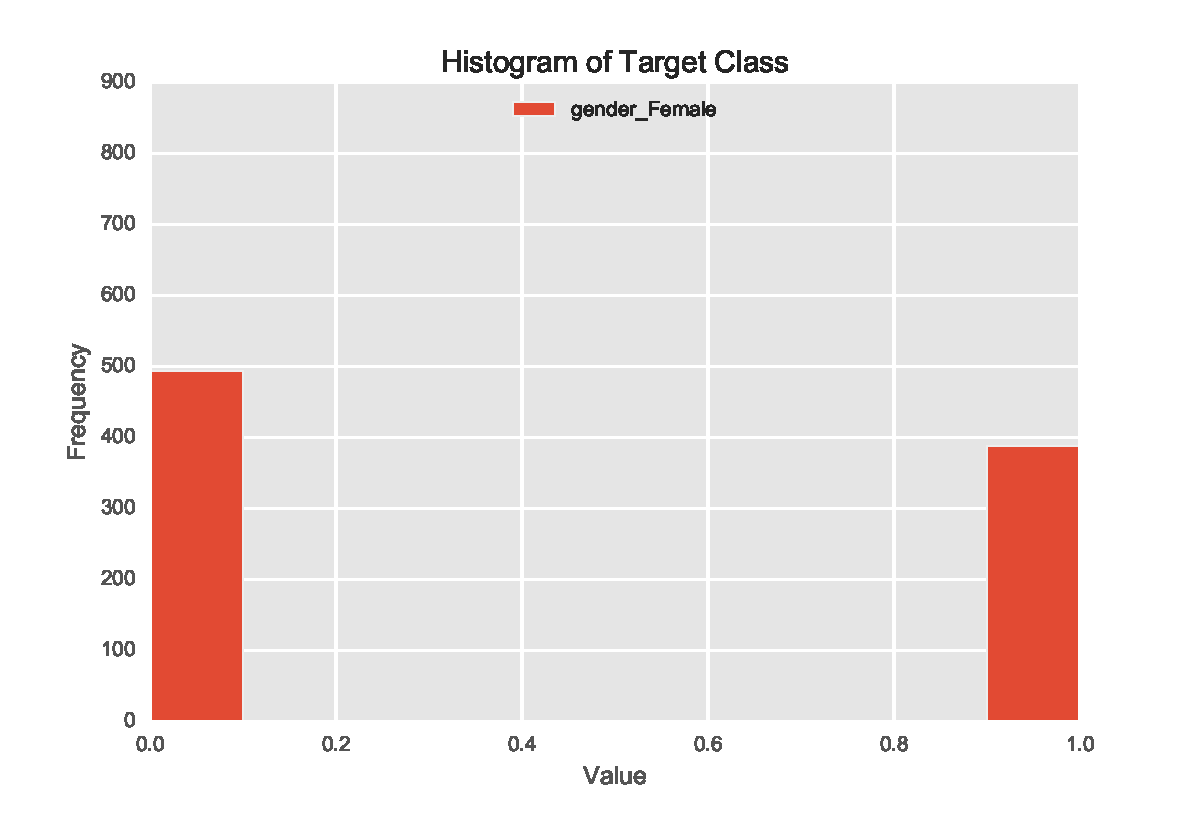
\includegraphics[width=1\textwidth]{figures/targetClass}
    \label{targetClass}
\end{figure}

\begin{figure}[!hbtp]
\centering

    \caption{\textbf{Expected Value Equation. }\textit{Expected rates multiplied by the cost-benefit weighted by the class priors.}}

    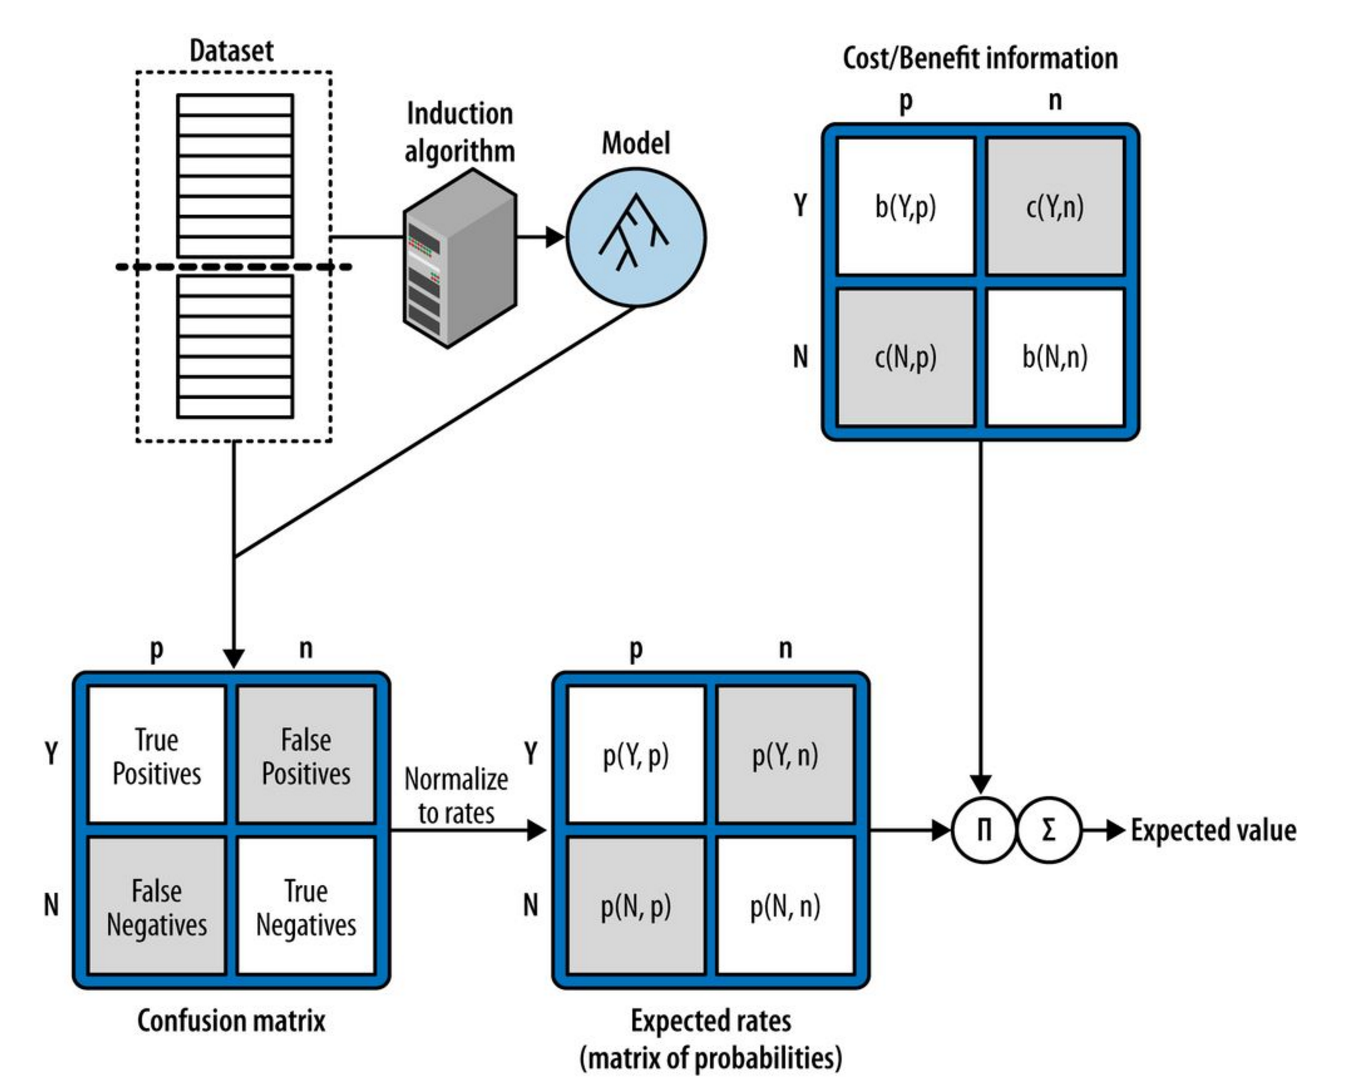
\includegraphics[width=1\textwidth]{figures/expectedValueCalculation.png}
    \label{expectedValue}
\end{figure}


%----------------------------------------------------------------------------------------
%  CHAPTER 
%----------------------------------------------------------------------------------------

\chapter*{Analysis}

\section* {Dataset}
The dataset used in this project consists of survey responses. A copy of the survey instrument can be found in the appendix of this report. The survey instruments were developed to measure participants' self-reported attitudes along several dimensions: 

\begin{enumerate}% 
\item \texttt{atcs}: CS beliefs
\item \texttt{atcsgender}: Gendered belief about CS ability
\item \texttt{atcsjob}: Career driven beliefs about CS
\item \texttt{atct}: Computational thinking beliefs
\item \texttt{blg}: CS belonging
\item \texttt{cltrcmp}: Collegiality
\end{enumerate}

In addition, the survey also collected data around student background: 

\begin{enumerate}% 
\item \texttt{prcs}: Prior collegiate CS exposure
\item \texttt{mtr}: CS mentors and role models
\item University demographics
\end{enumerate}



Majority of the questionnaire uses a 5-point Likert scale (where 1 = Strongly Disagree, 3 = Neutral and 5 = Strongly Agree). A code book was created to facilitate ease of analysis and interpretability of results. 

The dataset consists of 45 feature columns with 882 instances. Further, the dataset breakdowns into 494 male datapoints versus 388 female datapoints in the dataset. 


%----------------------------------------------------------------------------------------
%  CHAPTER 
%----------------------------------------------------------------------------------------



\section*{Missing Values}
The dataset with 45 features had two features with missing data.
\begin {itemize}    
\item priorcs10:                    43.88\% missing
\item reason\_class:                 0.68\% missing
\end{itemize} 

\section*{Data Preprocessing}

To prepare the data for classification, all features need to be transformed into numeric data. This dataset has several non-numeric columns that need converting. Many of them take on \texttt{yes} and \texttt{no} values, e.g. \texttt{prcs\_2}. These can be reasonably convert these into `1'/`0' (binary) values. For the columns whose values are `Nan', these will be converted to the mean of the column. Further, whitespaces will be removed from column names with the understanding that the tree plotting algorithm for Xgboost will fail if column names have spaces. 

The features were scaled using a minimax scaler to get better output for our SVM. This yielded the following values:
\begin {itemize}    
\item Strongly Disagree = 0.0
\item Disagree = 0.2
\item Neutral = 0.6
\item Agree = 0.8
\item Strongly Agree = 1.0
\end{itemize} 



\section*{Summarizing the data}
\begin{figure}[!hbtp]
\centering
    \caption{\textbf{Density estimation for dimension atcs. }\textit{Self-reported attitudes about CS.}}\label{atcs}
    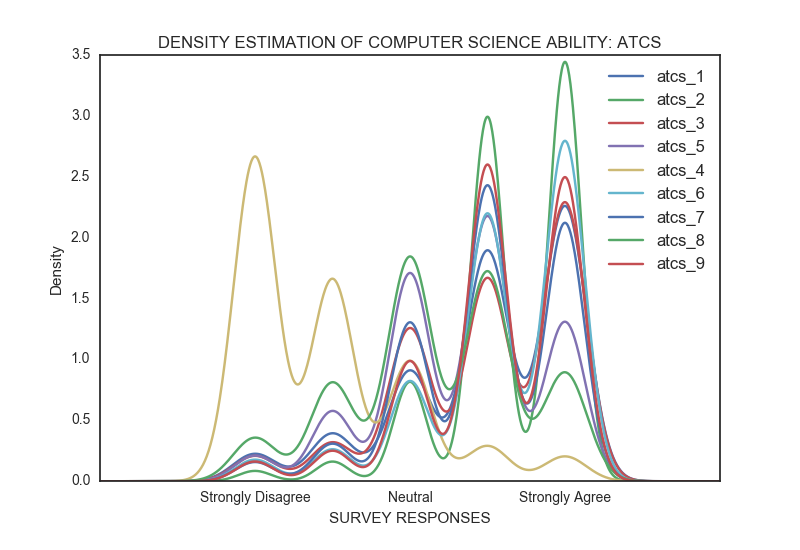
\includegraphics[width=0.8\textwidth]{figures/atcs}
\end{figure}
I created a density estimation for some dimensions in the data to gain an understanding of the variables and determine if I need to reject some of them, or collapse others. The distributions of most of the dimensions looked very similarly to that of \ref{atcs}. Most of the data is either skewed to the left or skewed to the right. As a result, I rejected using descriptive statistics to summarize the data in favor quantiles represented by box plots as can be seen in figure \ref{atcs_dimension}. 
\begin{figure}[!hbtp]
\centering
    \caption{\textbf{Quantiles for dimension \texttt{atcs. }}\textit{Self-reported attitudes about CS.}}\label{atcs_dimension}
    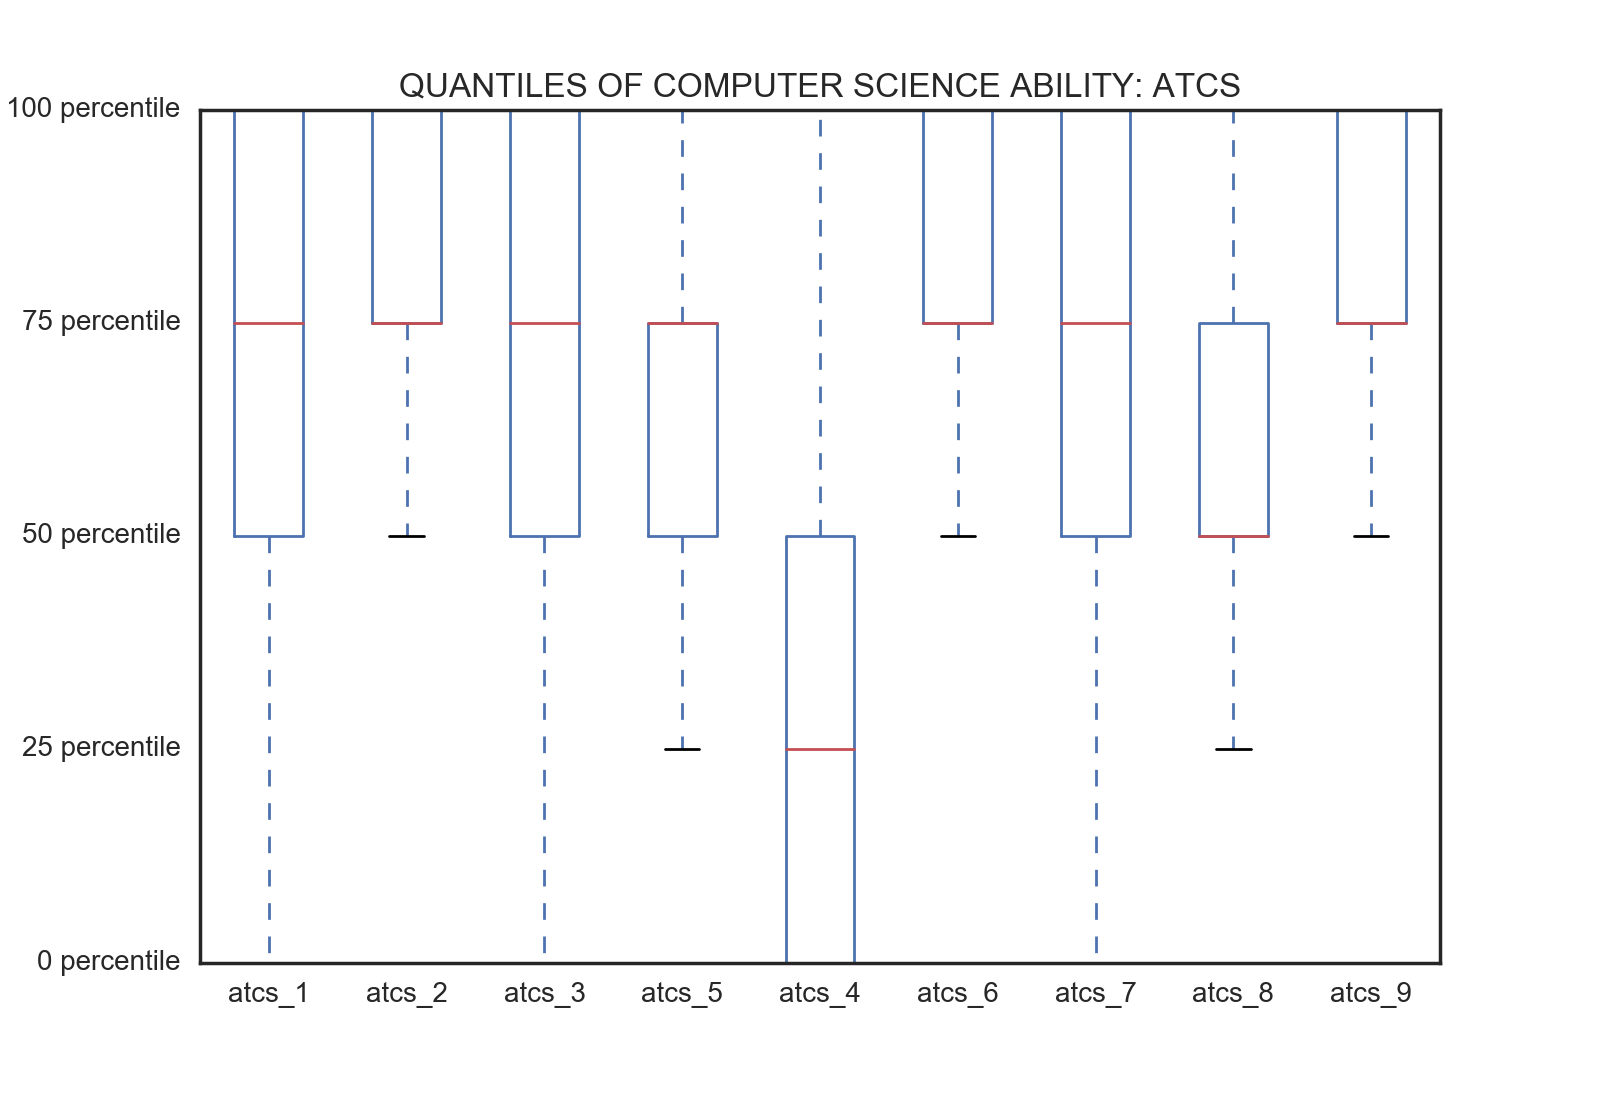
\includegraphics[width=1\textwidth]{figures/atcs_quantile}
\end{figure}

So what does figure \ref{atcs_dimension} tell us about the data? From that figure, we can see that the median of this dimension is approximately at the 75 percentile, which based on our Likert scale dataset means most students generally agree with the mostly positive attitudinal questions asked about their CS beliefs. For computational thinking, from figure \ref{atct_dimension} we see that most of the data in this dimension follow a similar distribution.
\begin{figure}[!hbtp]
\centering
    \caption{\textbf{Quantiles for dimension \texttt{atct.} }\textit{Self-reported attitudes about computational thinking.}}\label{atct_dimension}
    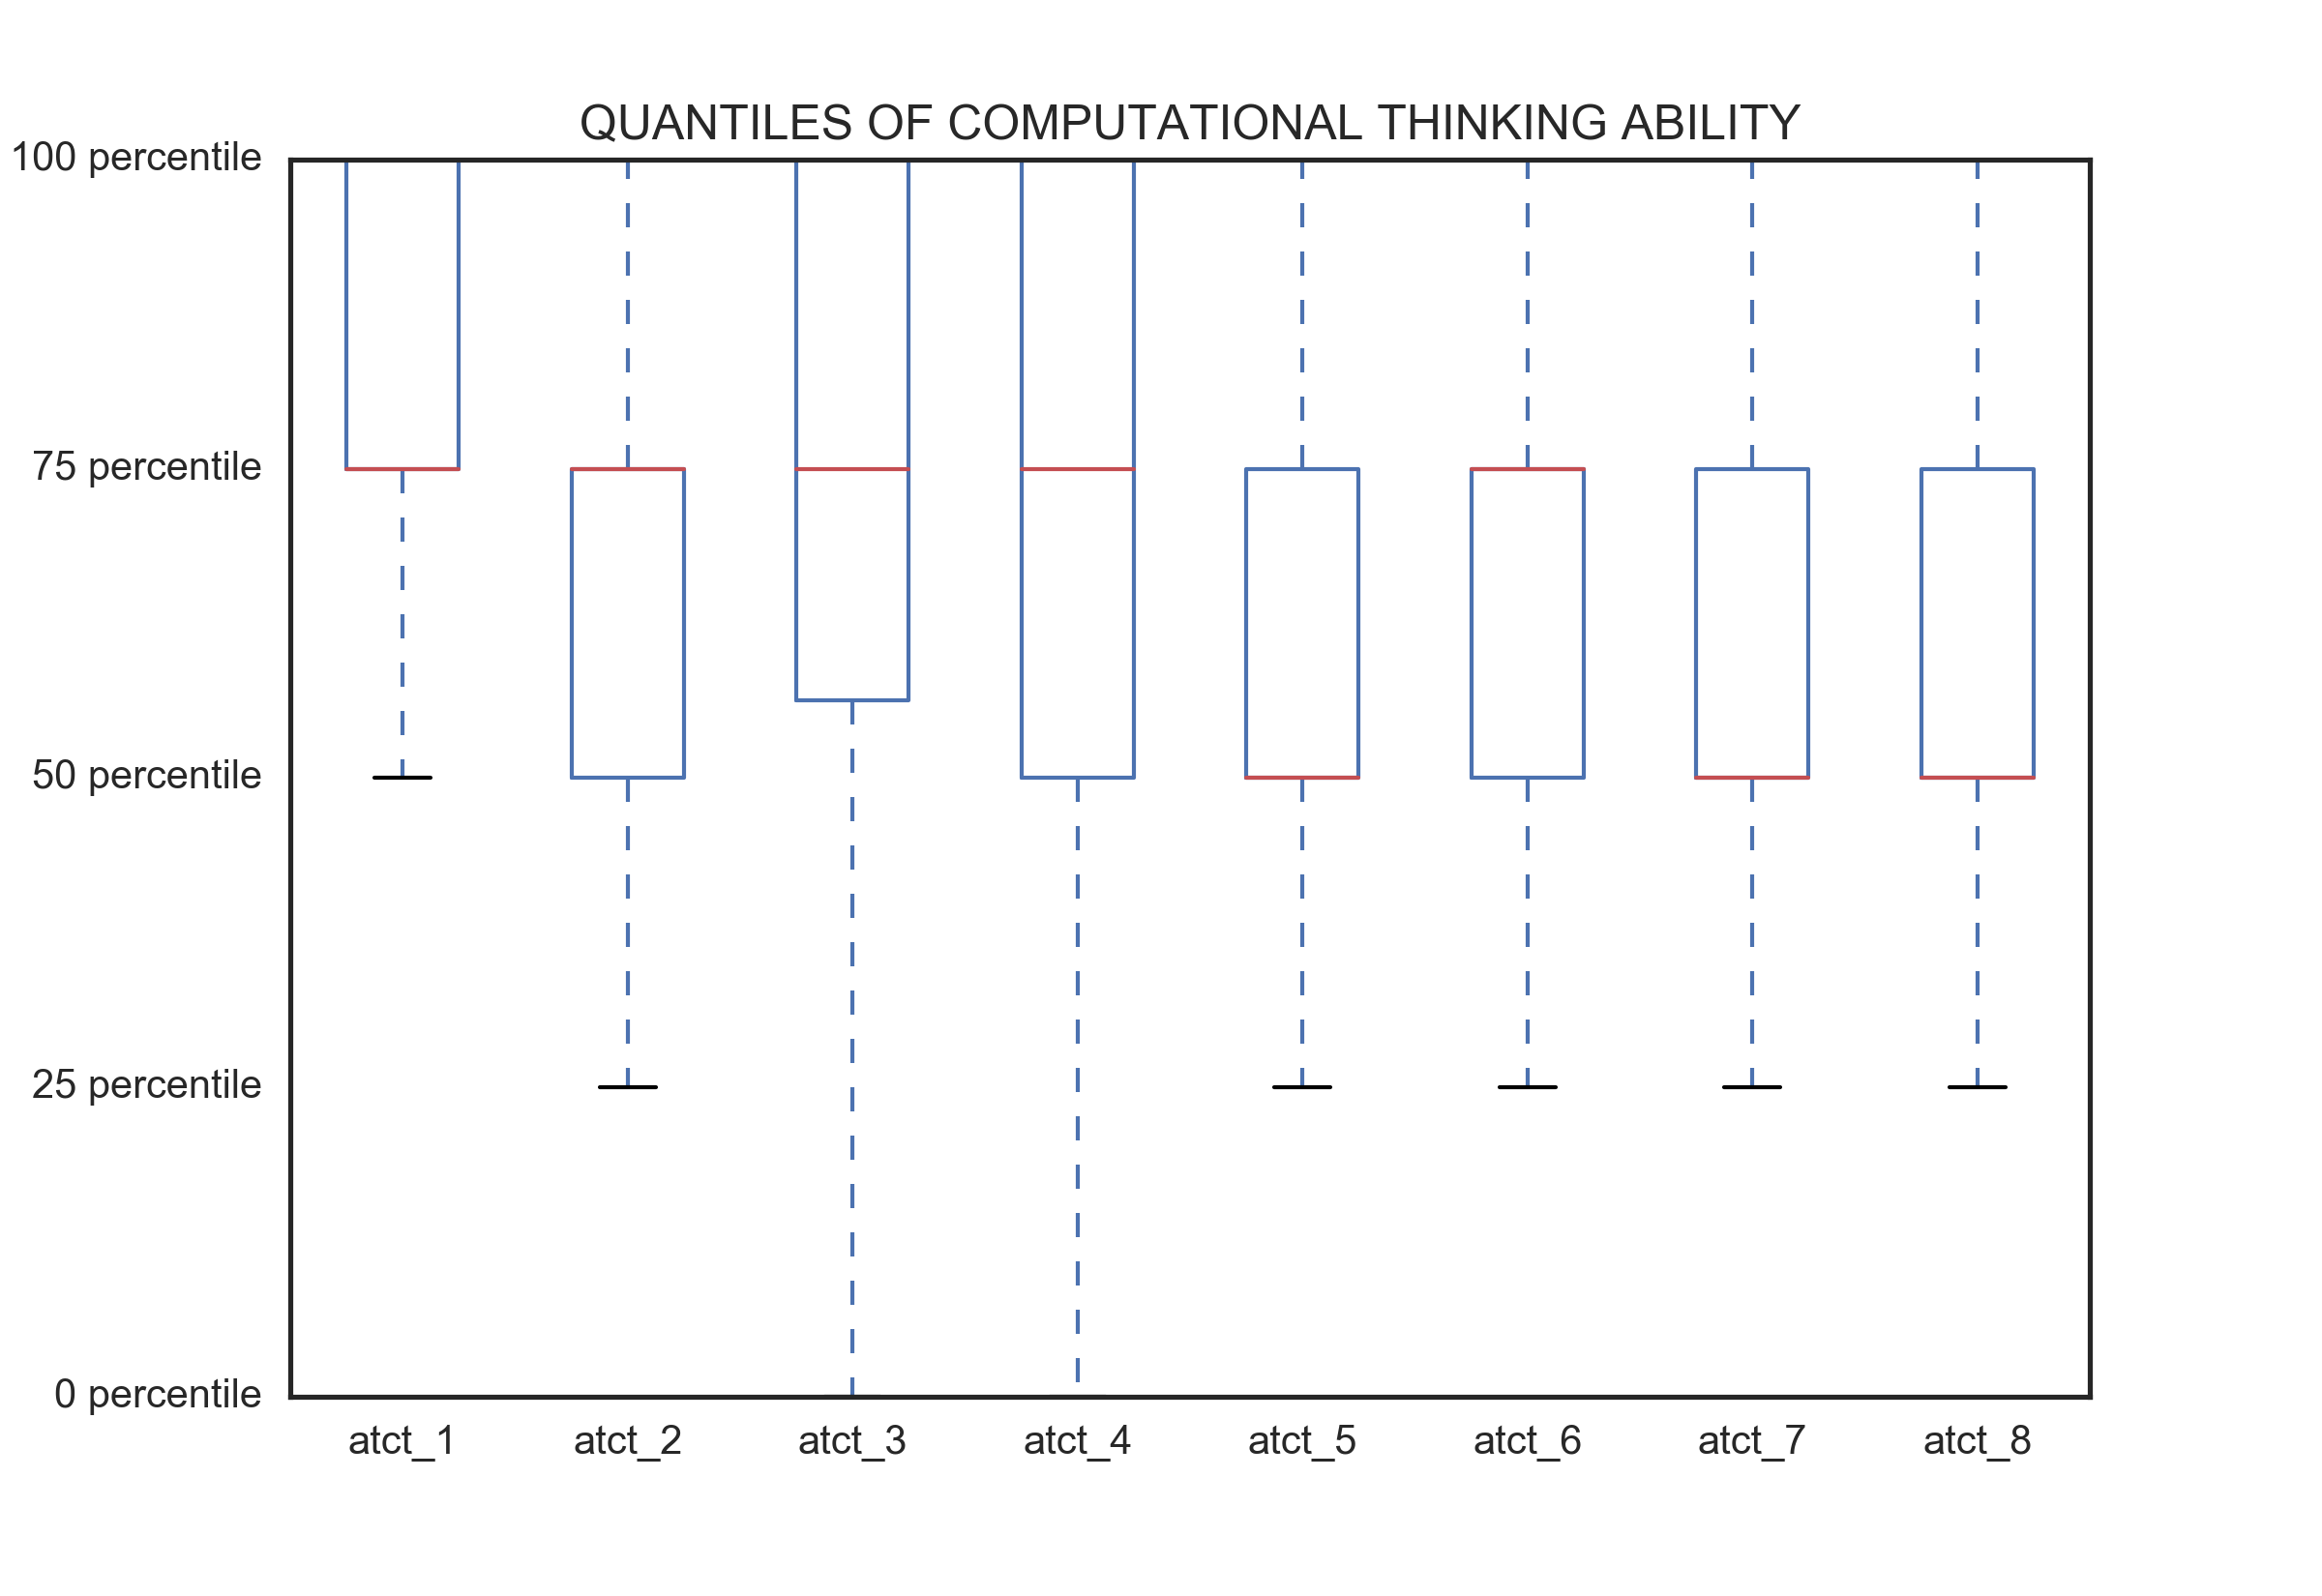
\includegraphics[width=1\textwidth]{figures/atct_quantile}
\end{figure}

From \ref{atcsgender}, I can see that the distribution for the dimension \texttt{atcsgender} is really skewed to the right, i.e., most students \emph{strongly disagree} with the statements. That does not come as a surprise, what I found fascinating is that the median for \texttt{atcsgender\_2} is at the 25 percentile, which corresponds to ``neutral.'' You can see this in the boxplot in figure \ref{atcsgender_quantile}.  While students do not agree that women are smarter than men, half of them are undecided about this statement!
\begin {itemize}
\item atcsgender\_1: Women are less capable of success in CS than men.
\item atcsgender\_2: Women are smarter than men.
\item atcsgender\_3: Men have better math and science abilities than women.
\end{itemize} 

\begin{figure}[!hbtp]
\centering
    \subfloat[]{%
    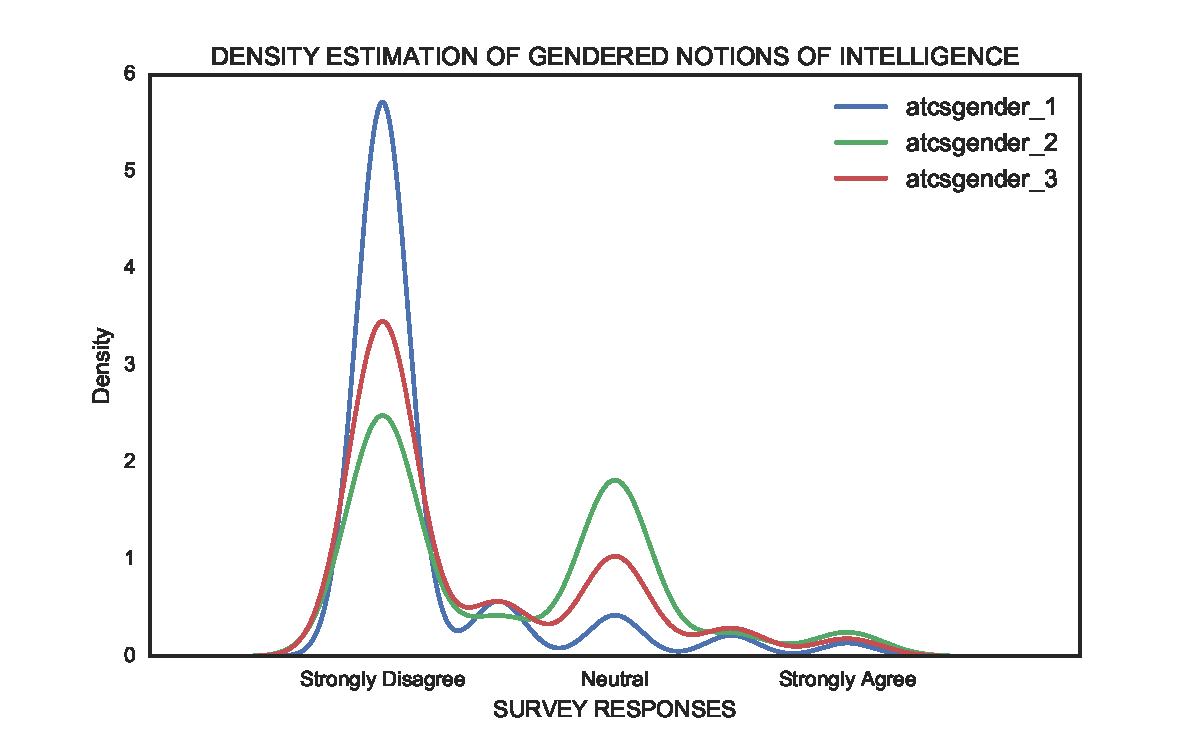
\includegraphics[width=0.6\textwidth]{figures/atcsgender}
    \label{atcsgender}}
    \subfloat[]{%
    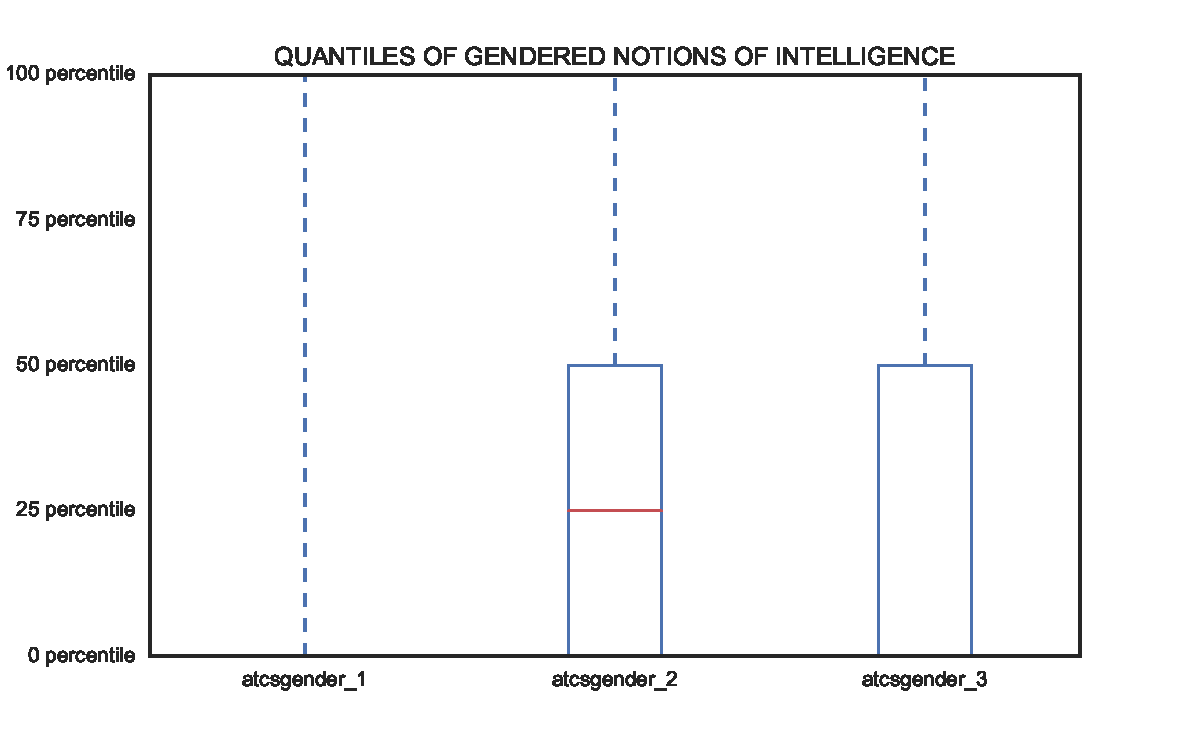
\includegraphics[width=0.6\textwidth]{figures/atcsgender_quantile}
    \label{atcsgender_quantile}}

    \caption{\textbf{Dimensions of \texttt{atcsgender}.} \textit{Figure (a) Density estimation for the dimension. Figure (b) Boxplot for the same dimension.}}
\end{figure}



\section*{Algorithms and Techniques}

For the problem of determining the factors that predict intro CS experience based on gender, I experimented with four different classifiers, a decision tree classifier, two ensemble methods and a support vector machine:

\begin{enumerate}% 
\item I selected a Random Forest classifier because it is considered one of the best off-the-shelf learning algorithm, and requires almost no tuning. 

\item I selected an eXtreme Gradient Boosted (XGBoost) trees classifier; which is an advanced implementation of the gradient boosting algorithm. From reading literature on machine learning in practice, the XGBoost classifier has differentiated itself as a classifier that has successfully demonstrated its performance in a wide range of problems. For example, ``among the 29 challenge winning solutions published at Kaggle's blog during 2015, 17 solutions used XGBoost.''

\item I selected a Support Vector Machine (SVMs) because they are very robust classifiers and \textit{more importantly}, they have a method to correct for class imbalances. 
              
\item Finally I selected a Decision Tree classifier because it lends itself to interpretability. For this problem domain, it is not just satisfactory for me to discriminate between male and female students, what I ultimately want is to gain \textit{insights} into what the salient factors around the experience of intro CS are, based on gender.

\end{enumerate}

\section*{Benchmark}

Before I start selecting which classifier I want to proceed with, I need a \textbf{baseline} score on which I can evaluate the practical value of datamining for this problem. Since this project is applying machine learning to a novel dataset, I do not have standard benchmarks I can measure against. As such, I have decided to use a simple \textit{majority} classifier which always selects the majority class of the training set. 

\section*{Implementation}
I implemented the four learning algorithms. For each of the learners I implemented the baseline algorithm using a stratified shuffle split cross validation with 10 folds and calculated the $F_1$ scores and looked at the confusion matrices respectively. 


\setlength{\extrarowheight}{1.5pt}
\begin{table}[!htbp]
\caption{Scores} %title of the table
\centering % centering table
\begin{tabular}{|l|l|l|r|} % creating four columns 
\hline % inserts single-line


\multicolumn{4}{|c|}{}\\
\multicolumn{4}{|c|}{Result of training the baseline classifiers}\\[5pt]
\hline
Classifier & Training Score & Prediction Score & Expected Value\\[0.5ex]
\hline % inserts single-line

Majority & - & 58.01\% & 0.0 \\
SVC     & 55.39\% & 53.57\% & 1.63\% \\
DecisionTree       & 51.08\% & 62.44\% & 2.63\%\\
RandomForestClassifier   & 54.93\% & 55.91\% & 1.87\%\\
XGBClassifier            & 59.69\% & 70.35\% & 3.11\%\\

\hline% inserts single-line
\end{tabular}
\label{tableBenchMarkScores}{}
\end{table}

From running these baseline classifiers, I selected the xgboost classifier, \ref{XGBCM}, as the right learner for this problem because it had the highest expected value score.

Its interesting to note that the Decision Tree classifier, \ref{DTCM}, had the highest true positive rate at 0.63, however, its false positive rate was a staggering 0.38! This means that it cannot find a meaningful sets of conditions for separating males from females in the dataset. The Support Vector Machine had the lowest false positive rate but did not beat the majority classifier because its true positive rate was abysmal. Where as, XGBoost does satisfactory on both fronts.

\begin{figure}[!hbtp]
\centering
    \subfloat[Random Forest]{%
    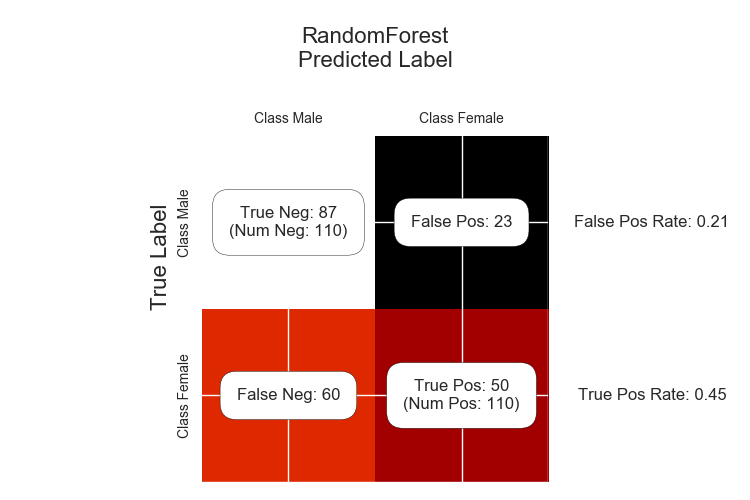
\includegraphics[width=0.65\textwidth]{figures/RandomForest}
    \label{RFCM}}
    \subfloat[Decision Tree]{%
    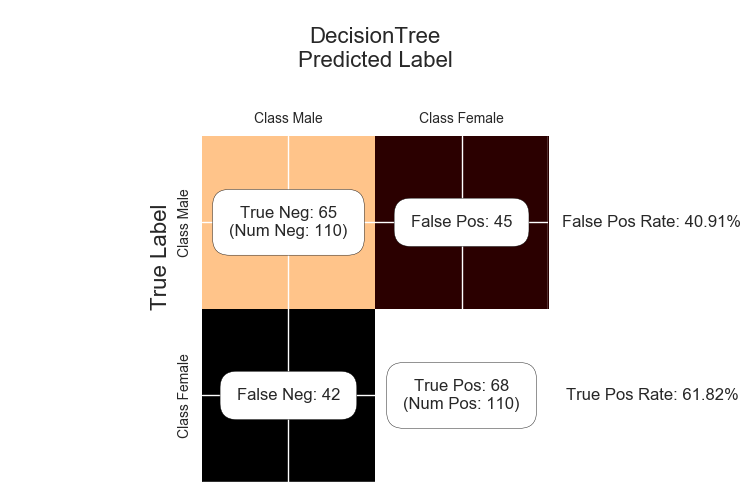
\includegraphics[width=0.65\textwidth]{figures/DecisionTree}
    \label{DTCM}}

    \quad


    \subfloat[XgBoost]{%
    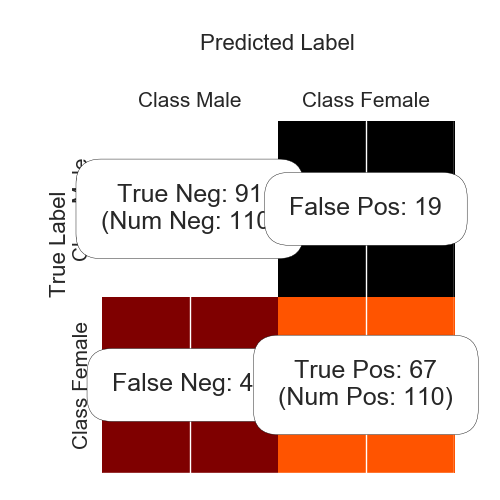
\includegraphics[width=0.65\textwidth]{figures/XGBoost}
    \label{XGBCM}}
    \subfloat[SVC]{%
    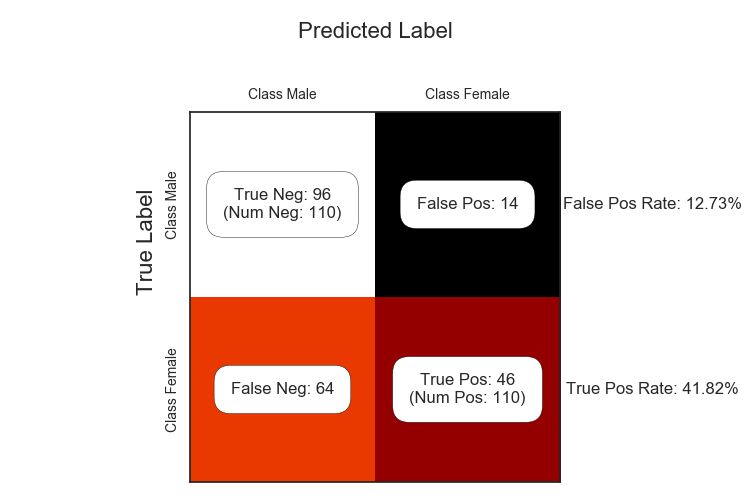
\includegraphics[width=0.65\textwidth]{figures/SVC}
    \label{SVCCM}}

    \caption{\textbf{Confusion Matrices of Baseline Classifiers}}
\end{figure}


%----------------------------------------------------------------------------------------
%  CHAPTER 
%----------------------------------------------------------------------------------------

\chapter*{Results}


\section*{Model Evaluation and Validation}

I am going to tune my model based on some heuristics about the kinds of value ranges that are suitable for the hyper-parameters I want to learn. I will be using these values ranges for the hyper-parameters:

\begin{itemize}
\item Parameters for Tree Booster
    \begin{itemize}
        \item \texttt{colsample\_bytree}
        \begin{itemize}
            \item subsample ratio of columns when constructing each tree
            \item Range (0, 1], default 6, tuned on $[0.4, 0.6, 0.8, 1.0]$
        \end{itemize}
        \item \texttt{n\_estimators}
        \begin{itemize}
            \item Minimum number of trees
            \item Range $[2,\infty]$ default 2, tuned on $range(100, 1100, 100)$
        \end{itemize}

    \end{itemize}

\item Task Parameter
    \begin{itemize}
        \item \texttt{learning\_rate}
        \begin{itemize}
            \item Scale the contribution of each tree by learning rate
            \item Range $[0, 1]$, tuned on $[0.2222, 0.4444, 0.6666, 0.8888]$
        \end{itemize}
    \end{itemize}
\end{itemize}
I will implement the tuning using sklearn's \texttt{GridSearch} in conjunction with a \{k=50 fold\} \texttt{StratifiedShuffleSplit} function. 

\section*{Results of tuning}
Once I performed the search through the hyper-parameter space to find the combination of hyper-parameters that maximized the performance of the selected classifier, I was able to \textbf{improve} the previous $F_1$ score by \textbf{2.85\%}, to achieve a prediction score of 71.22\%.

From figures \ref{cfmatrix_base} and \ref{cfmatrix_tuned}, one can see that the \textbf{false negative} count for the female class has gone from 43 down to 37. This decision cost us a very small increase in the \textbf{false positive} count of the male class from 19 to 22. This is not too bad, so I will stick with this improved model.

\begin{figure}[!hbtp]
\centering
    \subfloat[Base Model]{%
    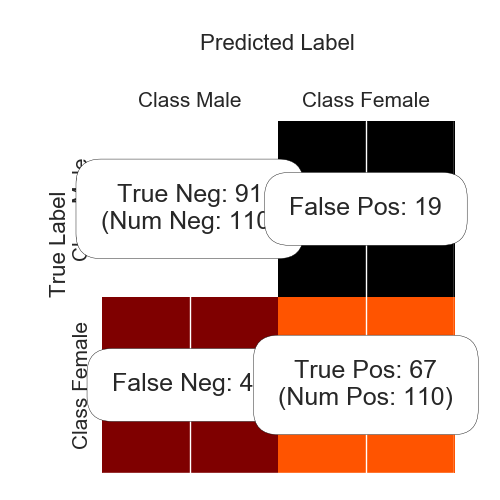
\includegraphics[width=0.65\textwidth]{figures/XGBoost}
    \label{cfmatrix_base}}
    \subfloat[Tuned Model]{%
    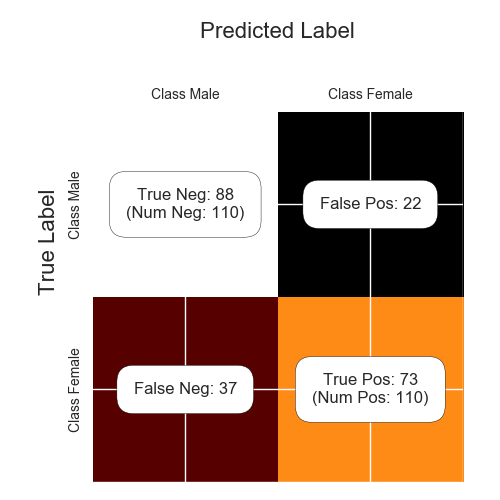
\includegraphics[width=0.65\textwidth]{figures/tuned_model_CM}
    \label{cfmatrix_tuned}}

    \caption{\textbf{Confusion Matrix}}
\end{figure}

Here is the final model for classifying gender in introductory CS. 
\begin{verbatim}
Best accuracy obtained: 71.22%
Parameters:
    n_estimators: 700
    subsample: 0.7
    learning_rate:  0.4444
    colsample_bytree: 0.6
    max_depth: 4

\end{verbatim}


\section*{Feature Importance}
There are two things that need consideration when using xgBoost for understanding feature importance: the features that are doing the \emph{most} work in splitting the data, and the automatically generated feature importance ranking that is done in by the xgBoost algorithm.

I plotted some estimators in the xgboost learner to see which features are doing the most work in splitting the data. I chose to focus on the \textbf{first} and \textbf{second} tree in the ensemble. On simple models, the first two trees may be enough to gain a \textit{strong} understanding. I then compare the output generated by these trees to the features generated by the model's own feature selection algorithm. 

From figures \ref{firstXGraph} and \ref{secondXGraph}, I see that 


\begin{figure}[!hbtp]
\centering
    \subfloat[First tree in the ensemble]{%
    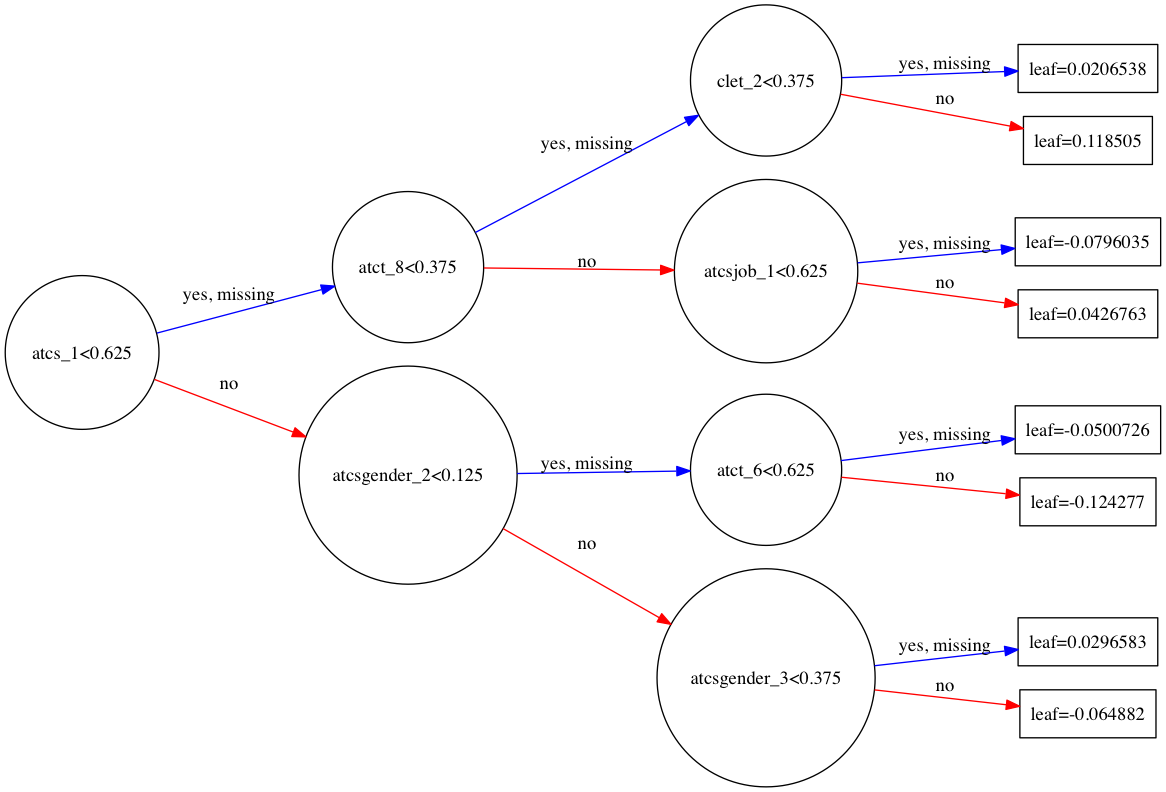
\includegraphics[width=0.5\textwidth]{figures/firstXGraph}
    \label{firstXGraph}}

    \subfloat[Second tree in the ensemble]{%
    \includegraphics[width=0.5\textwidth]{figures/secondXGraph}
    \label{secondXGraph}}

    \caption{\textbf{XgBoost base model decision trees}}
\end{figure}


\setlength{\extrarowheight}{1.5pt}
\begin{table}[!htbp]
\caption{Feature Importance} %title of the table
\centering % centering table
\begin{tabular}{|l|l|p{10cm}|} % creating four columns 
\hline % inserts single-line


\multicolumn{3}{|c|}{}\\
\multicolumn{3}{|c|}{XGBoost Feature Importance}\\[5pt]
\hline
Rank & Coded item & Description\\[0.5ex]
\hline % inserts single-line

1 & atcsgender\_2 &  Women are smarter than men. \\
2 & atcsjobs\_2 & My career goals do not require that I learn computing skills. \\
3 & clet\_2 &  I think about the ethical, legal, and social implications of computing.\\
4 & atct\_6 & I am good at building things.\\
5 & prepared & How prepared did you feel about this class before it started? \\
6 & atcsjob\_1 & Knowledge of computing will allow me to secure a good job. \\
7 & clet\_1 & I work well in teams. \\
8 & atct\_7 & I am good at ignoring irrelevant details to solve a problem. \\
9 & blg\_1 & In this class, I feel I belong. \\
10 & atct\_3 &  I am good at using online search tools. \\

\hline% inserts single-line
\end{tabular}
\label{tableFeatureImportance}{}
\end{table}

\subsection*{Optimized Trees}
I did not want the model to get overly complex because I wanted to make use of the tree as a set of rules; as such, I fixed the tree depth to 4 levels. Looking at figure \ref{first_tuned_tree}, you can see that this model as segmented the data into 14 distinct types because there are 14 nodes on the tree.
\begin{figure}[!hbtp]
\centering
    \subfloat[First tree in the ensemble]{%
    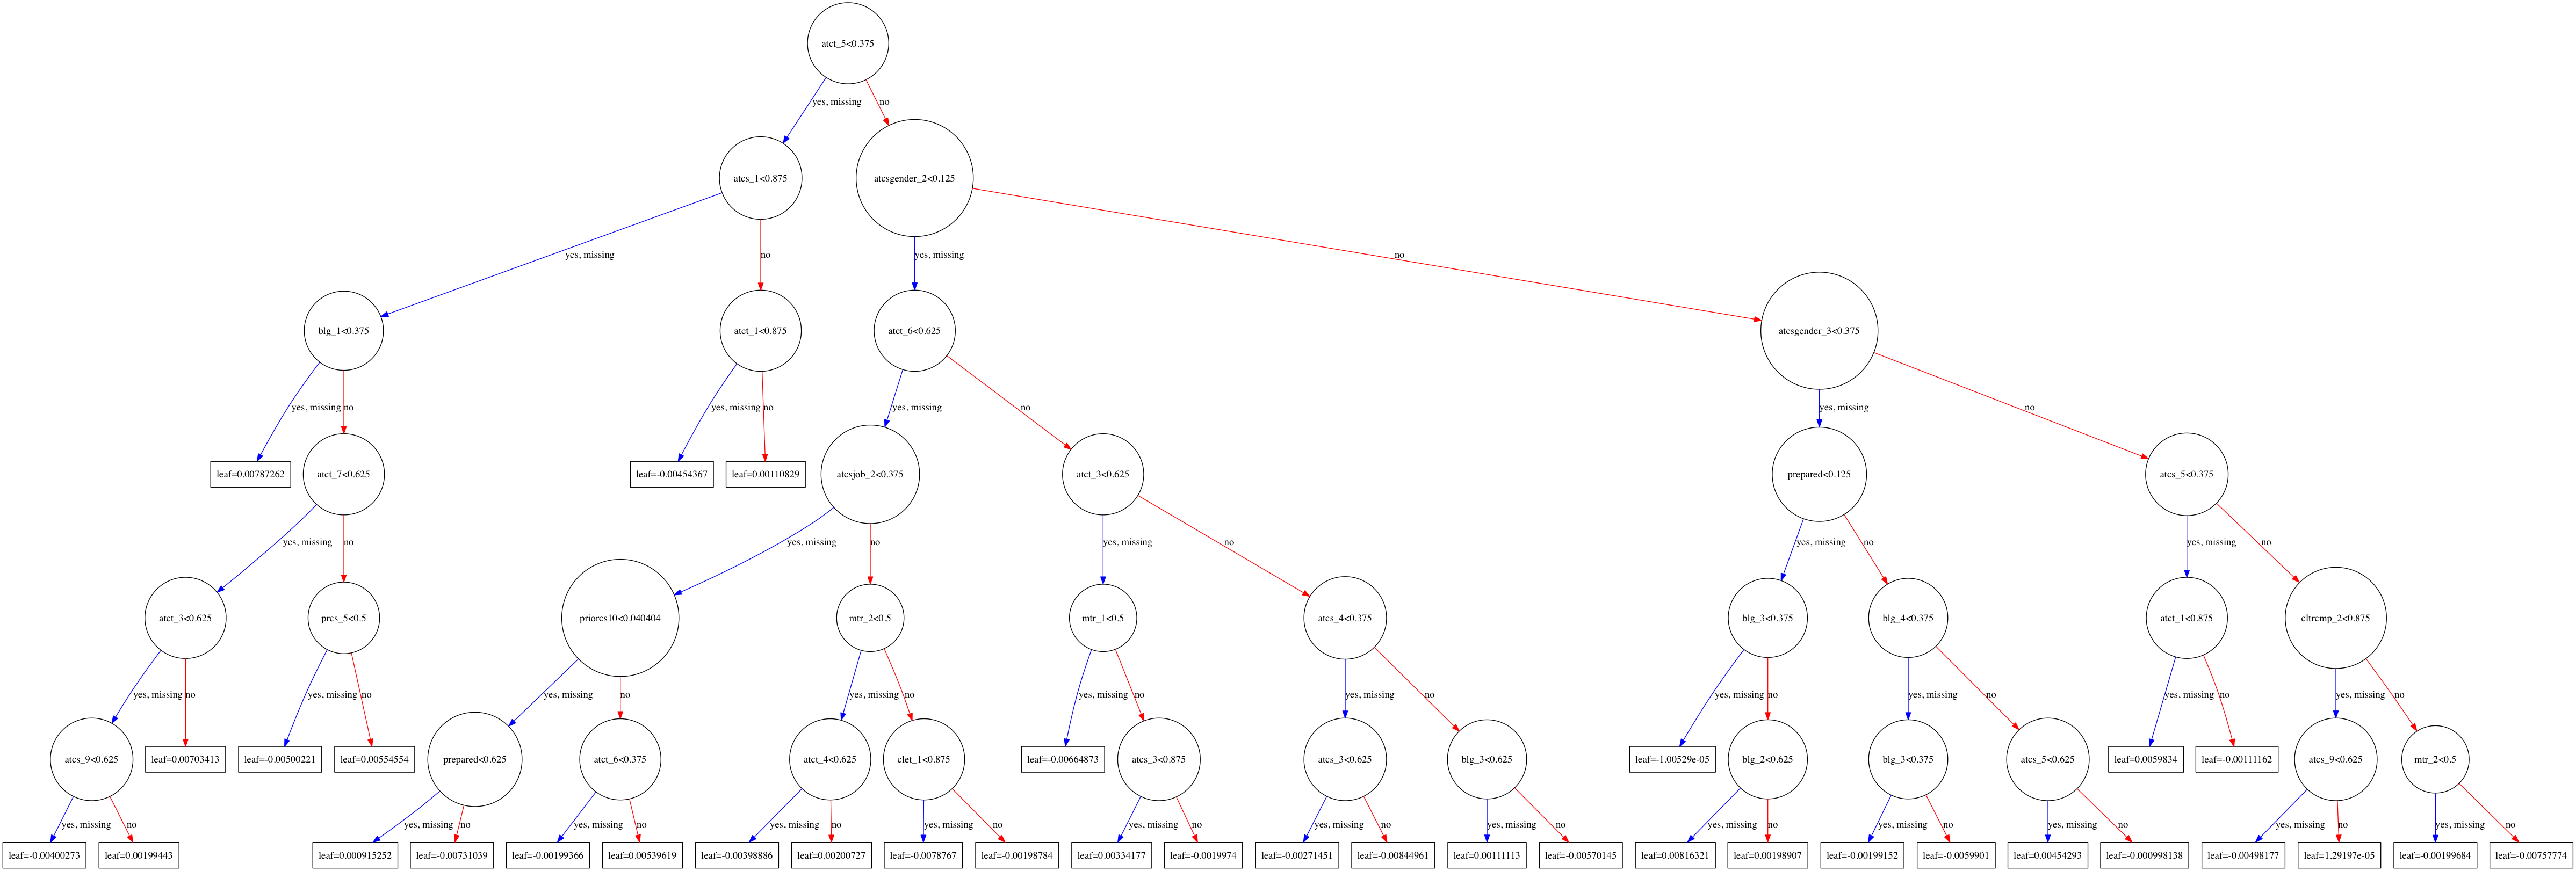
\includegraphics[width=1\textwidth]{figures/first_tuned_model_graph}
    \label{first_tuned_tree}}

    \qquad

    \subfloat[Second tree in the ensemble]{%
    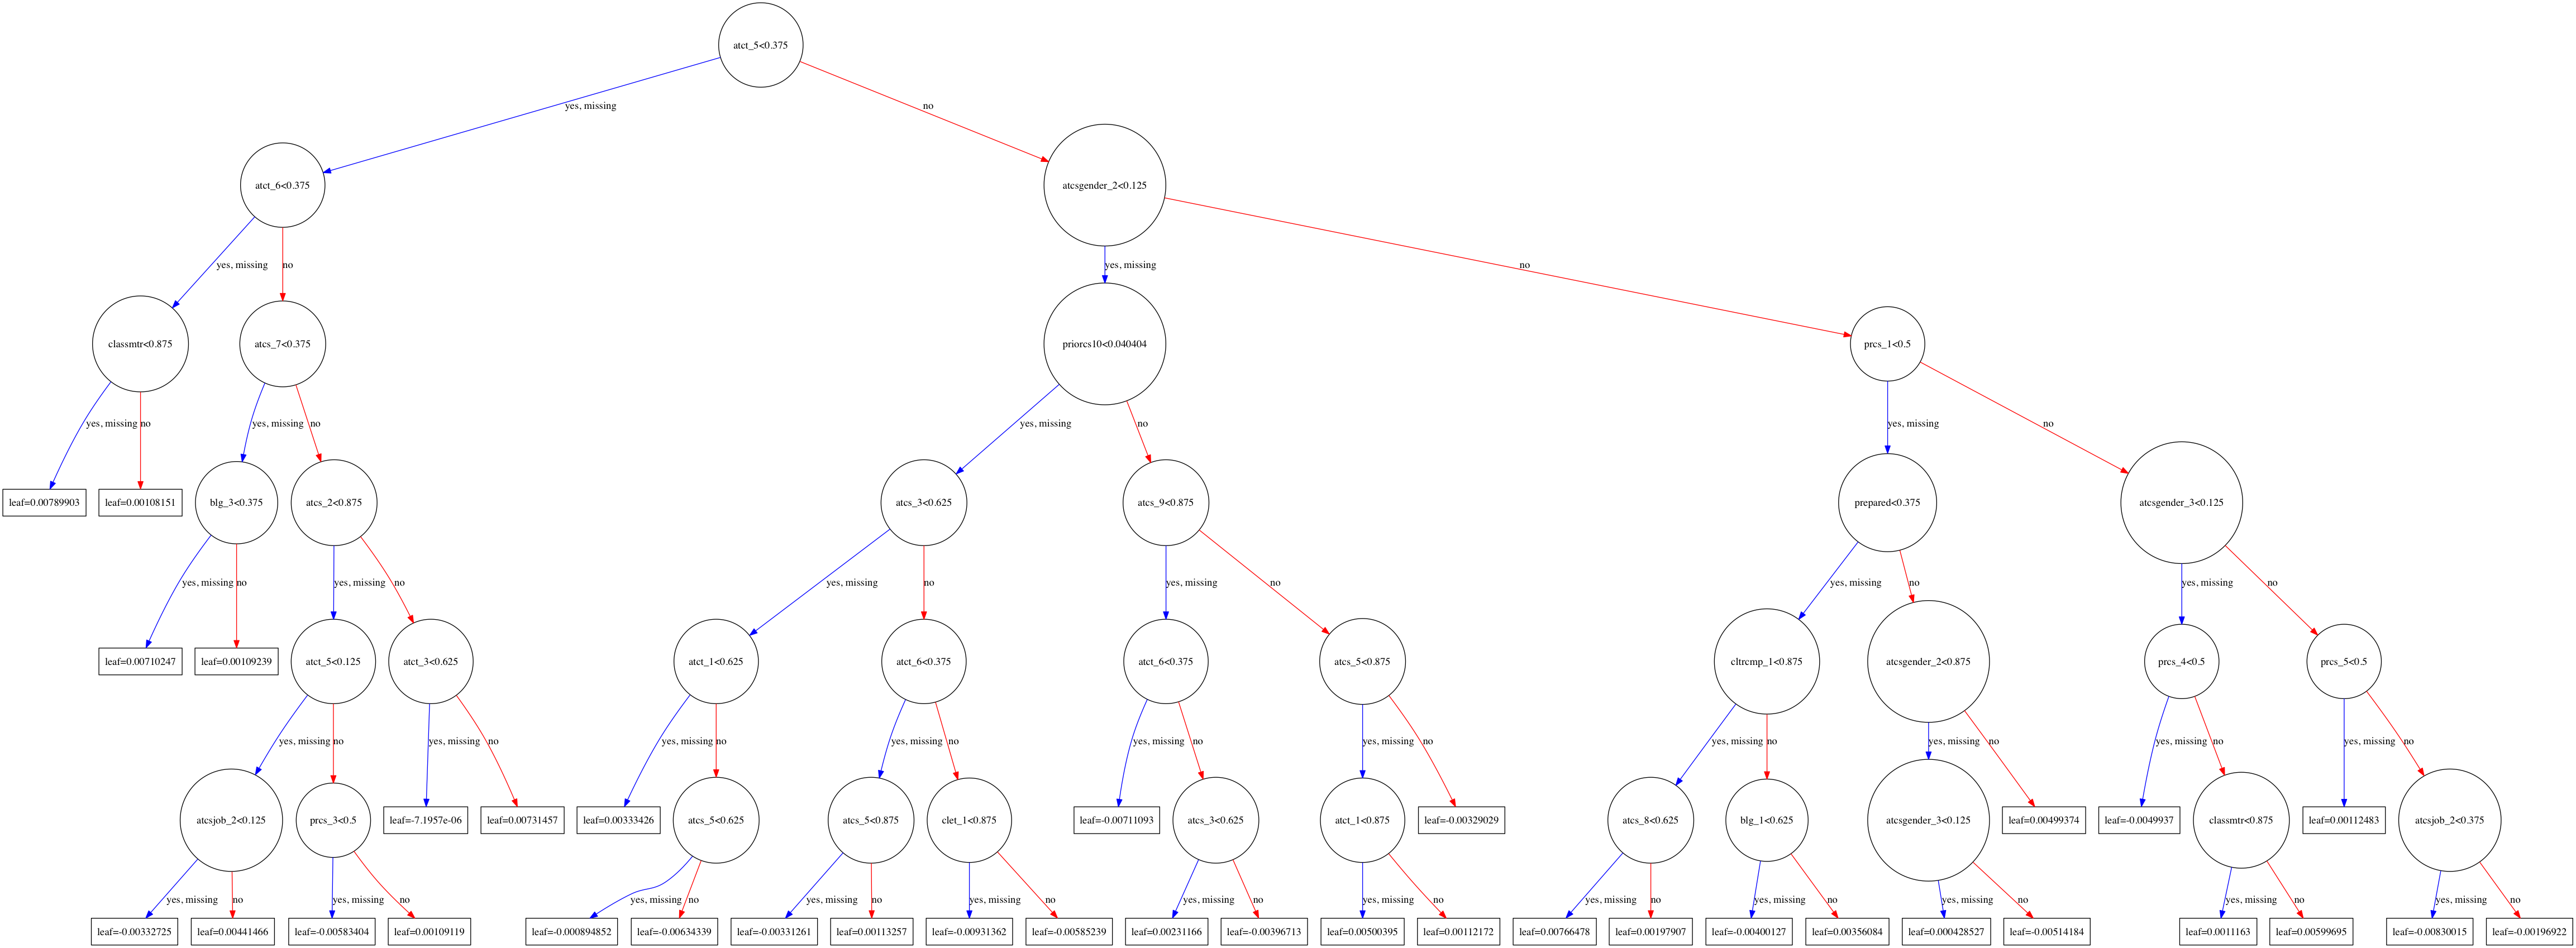
\includegraphics[width=1\textwidth]{figures/second_tuned_model_graph}
    \label{secondtuned_tree}}

    \caption{\textbf{Tuned XgBoost estimator decision tree.}}
\end{figure}


Information gain, lets us know how valuable a feature is in discriminating the dataset. That is, if we know the information gain of a feature, we can know how much it would contribute to the knowledge of the value of the target label. 

\begin{figure}[!hbtp]
\centering
    \subfloat[Feature Importance Base Model]{%
    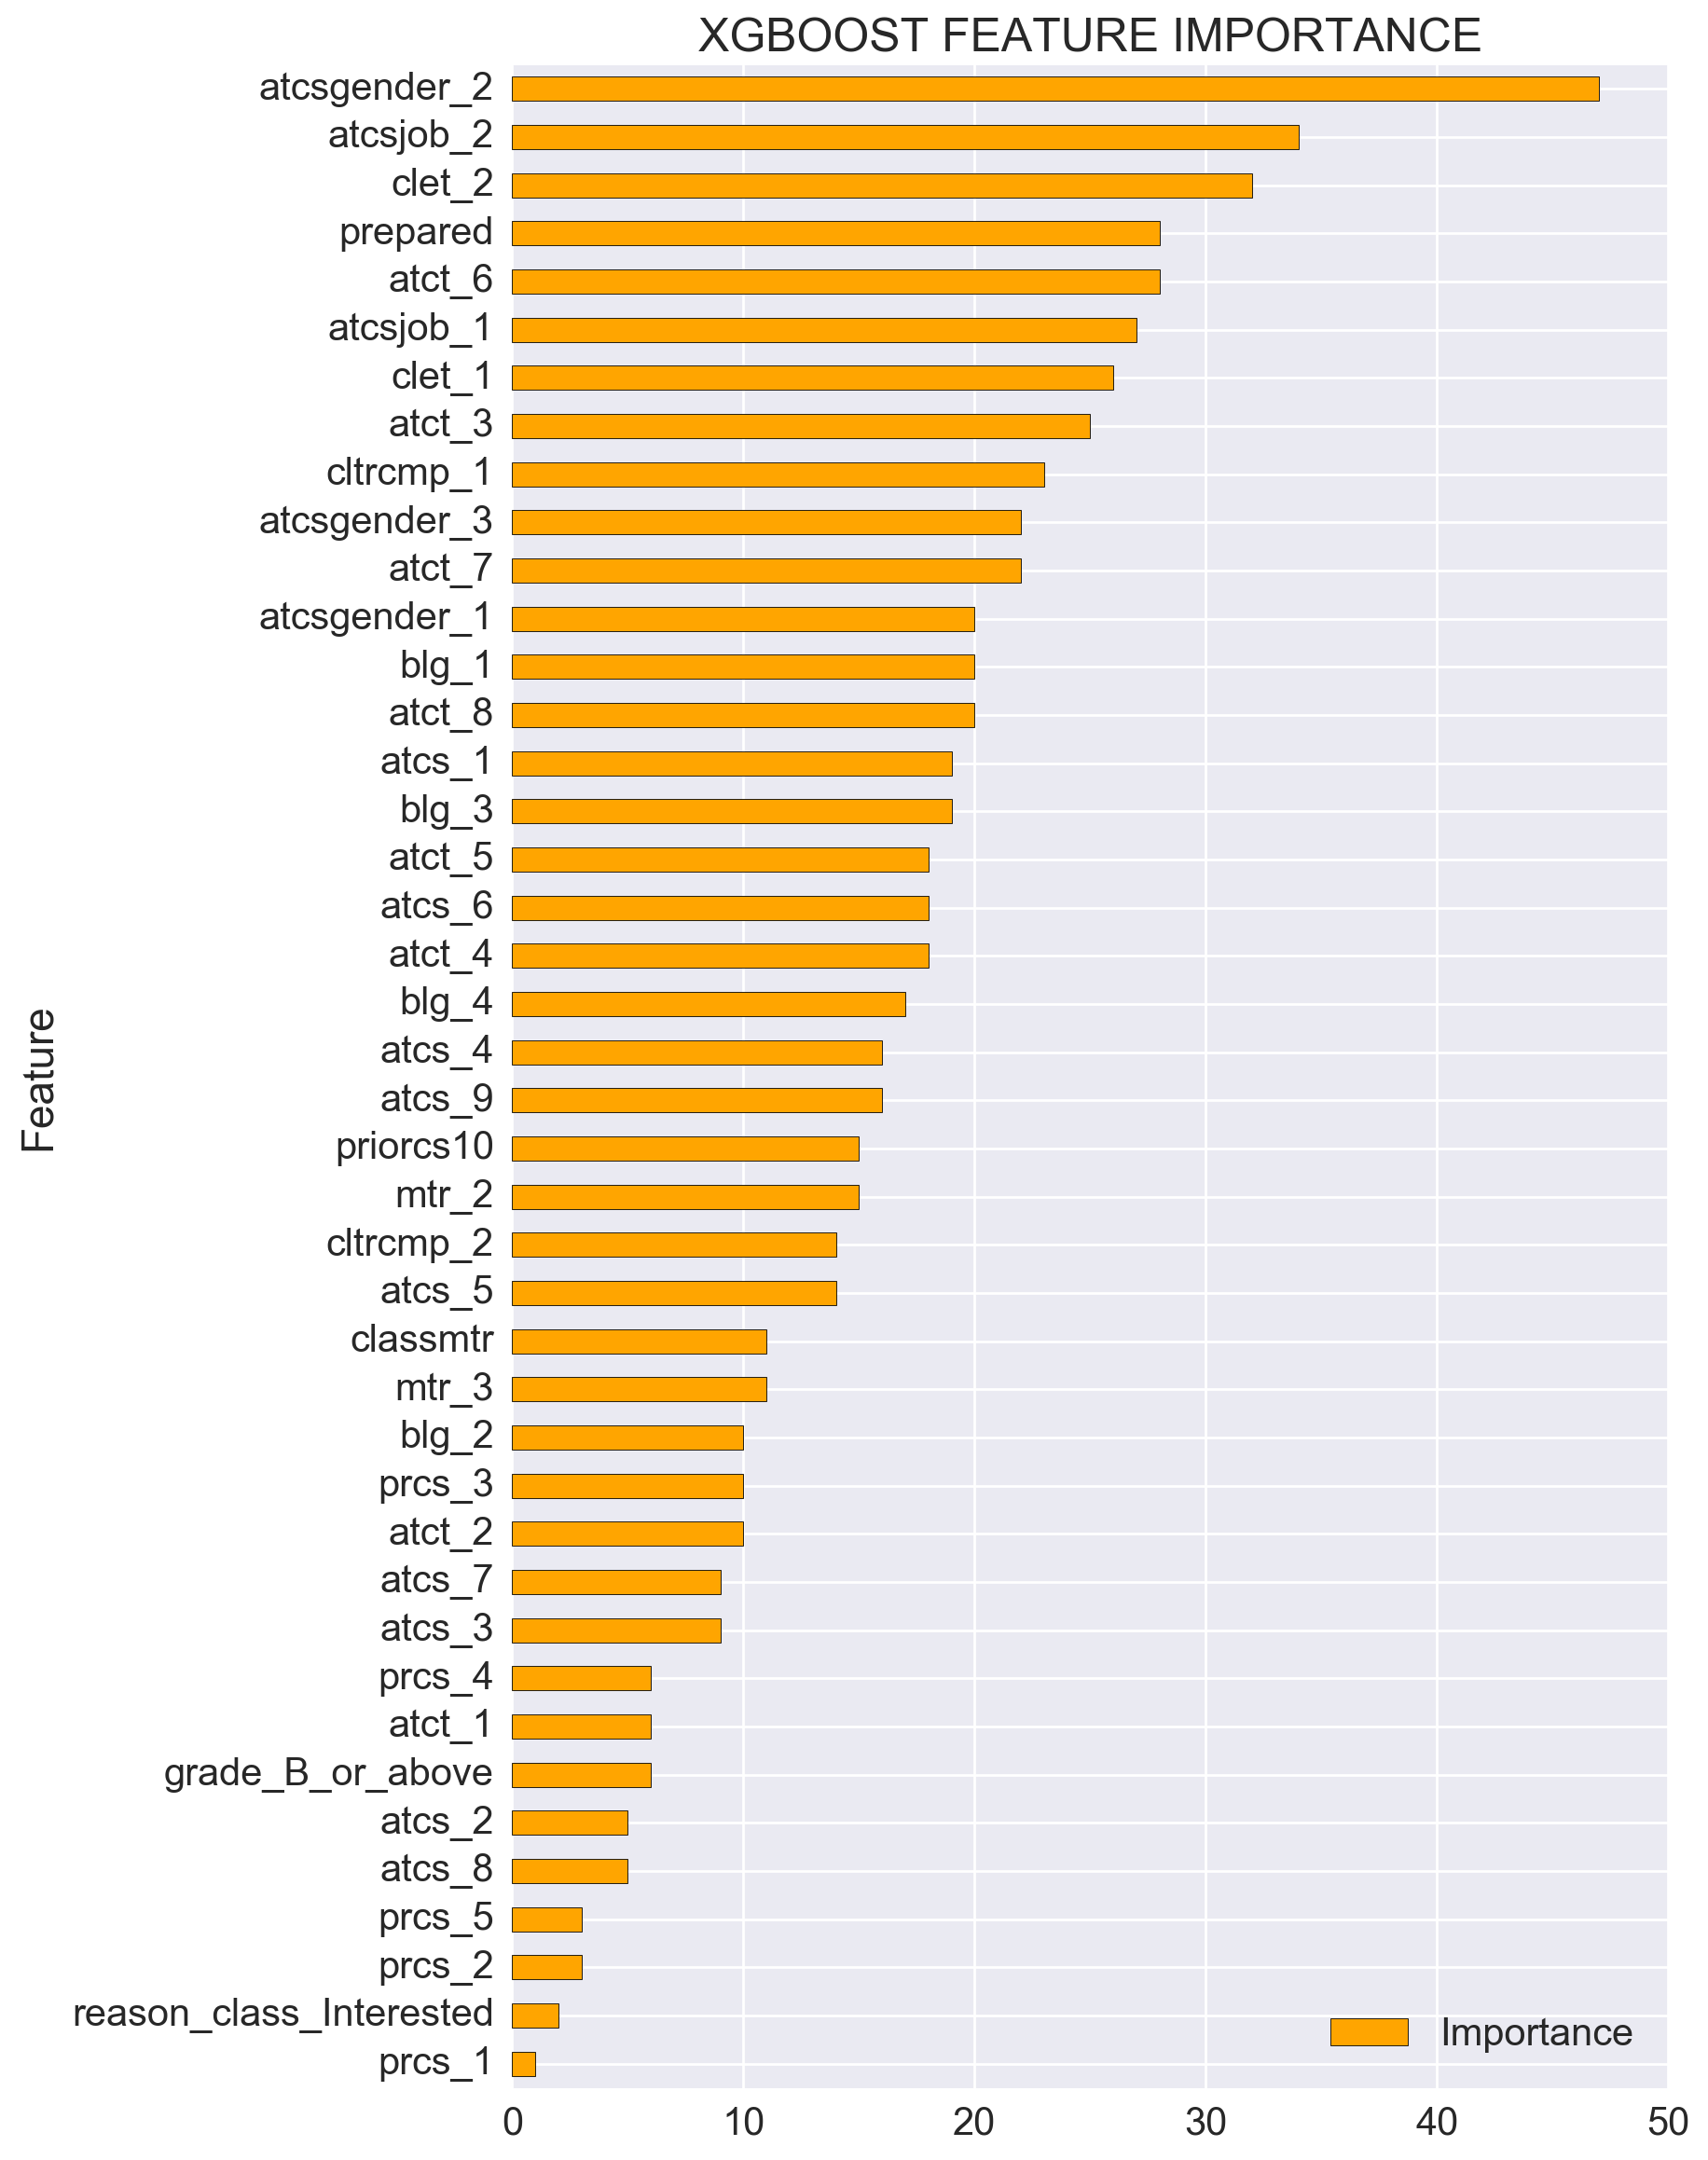
\includegraphics[width=0.6\textwidth]{figures/featureImportance}
    \label{f_imp}}
    \subfloat[Feature Importance Tuned Model]{%
    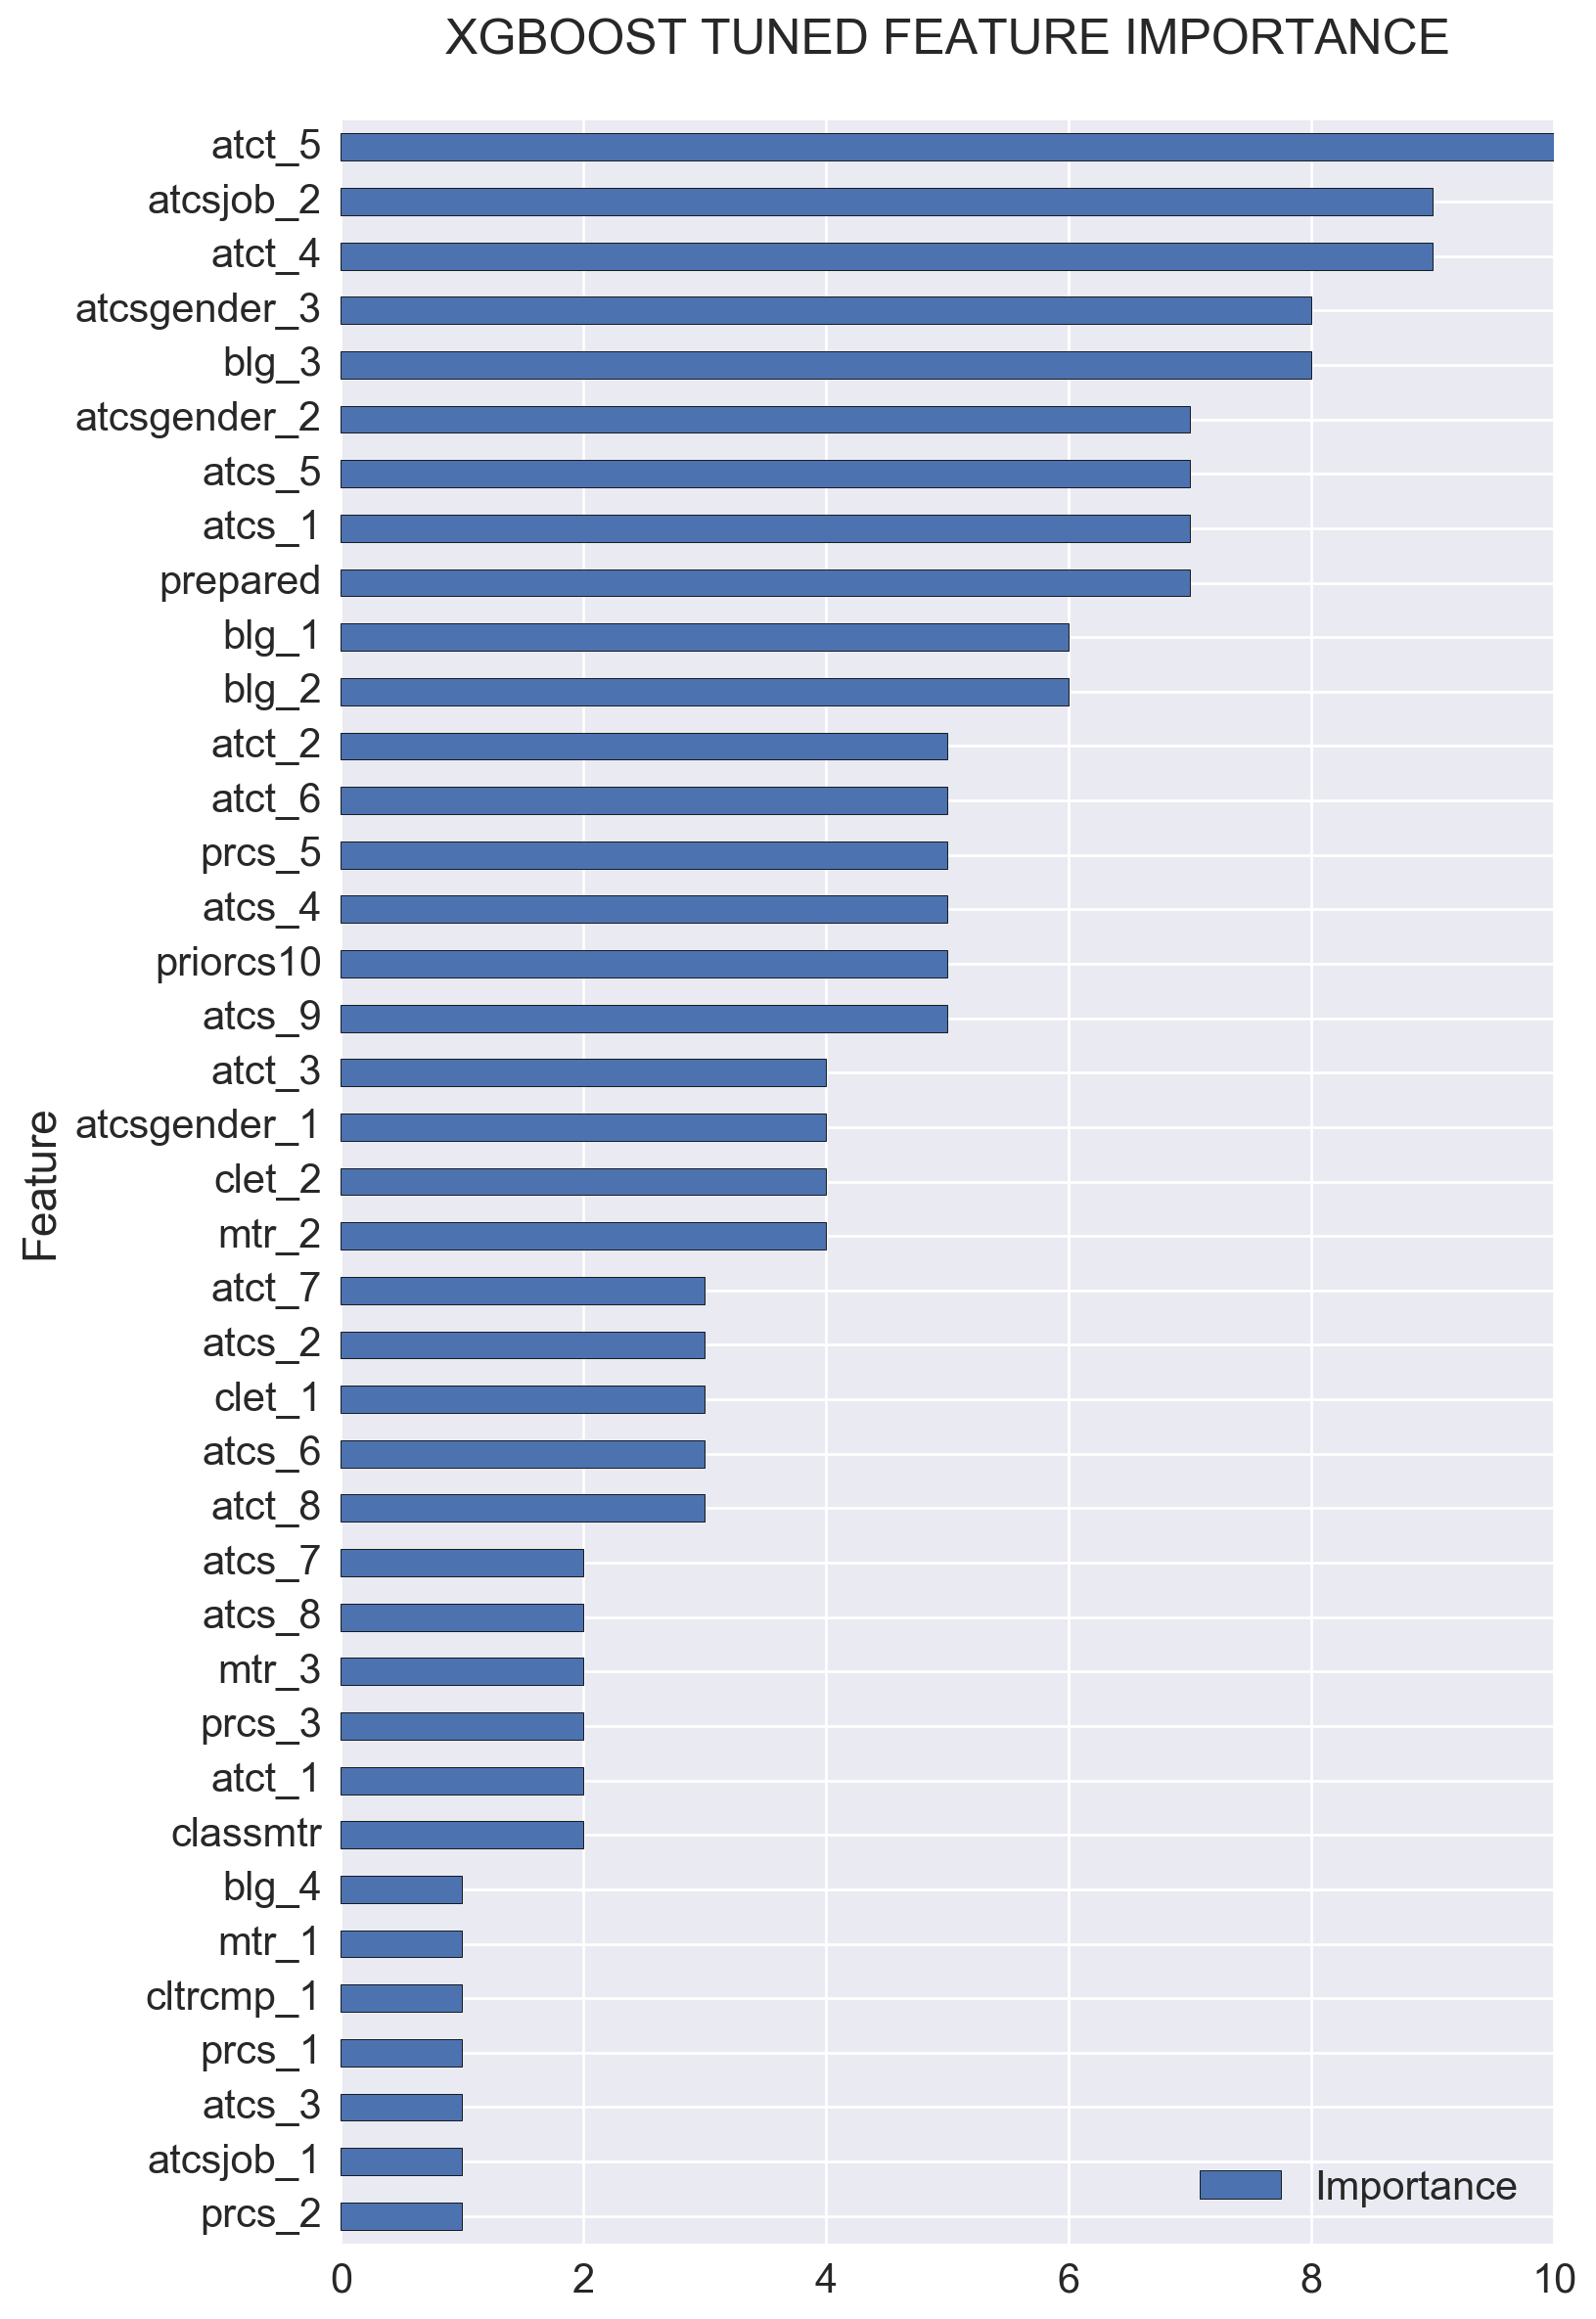
\includegraphics[width=0.6\textwidth]{figures/featureImportance_tuned}
    \label{f_imp_tuned}}

    \qquad

    \subfloat[Feature Importance Based on Cover]{%
    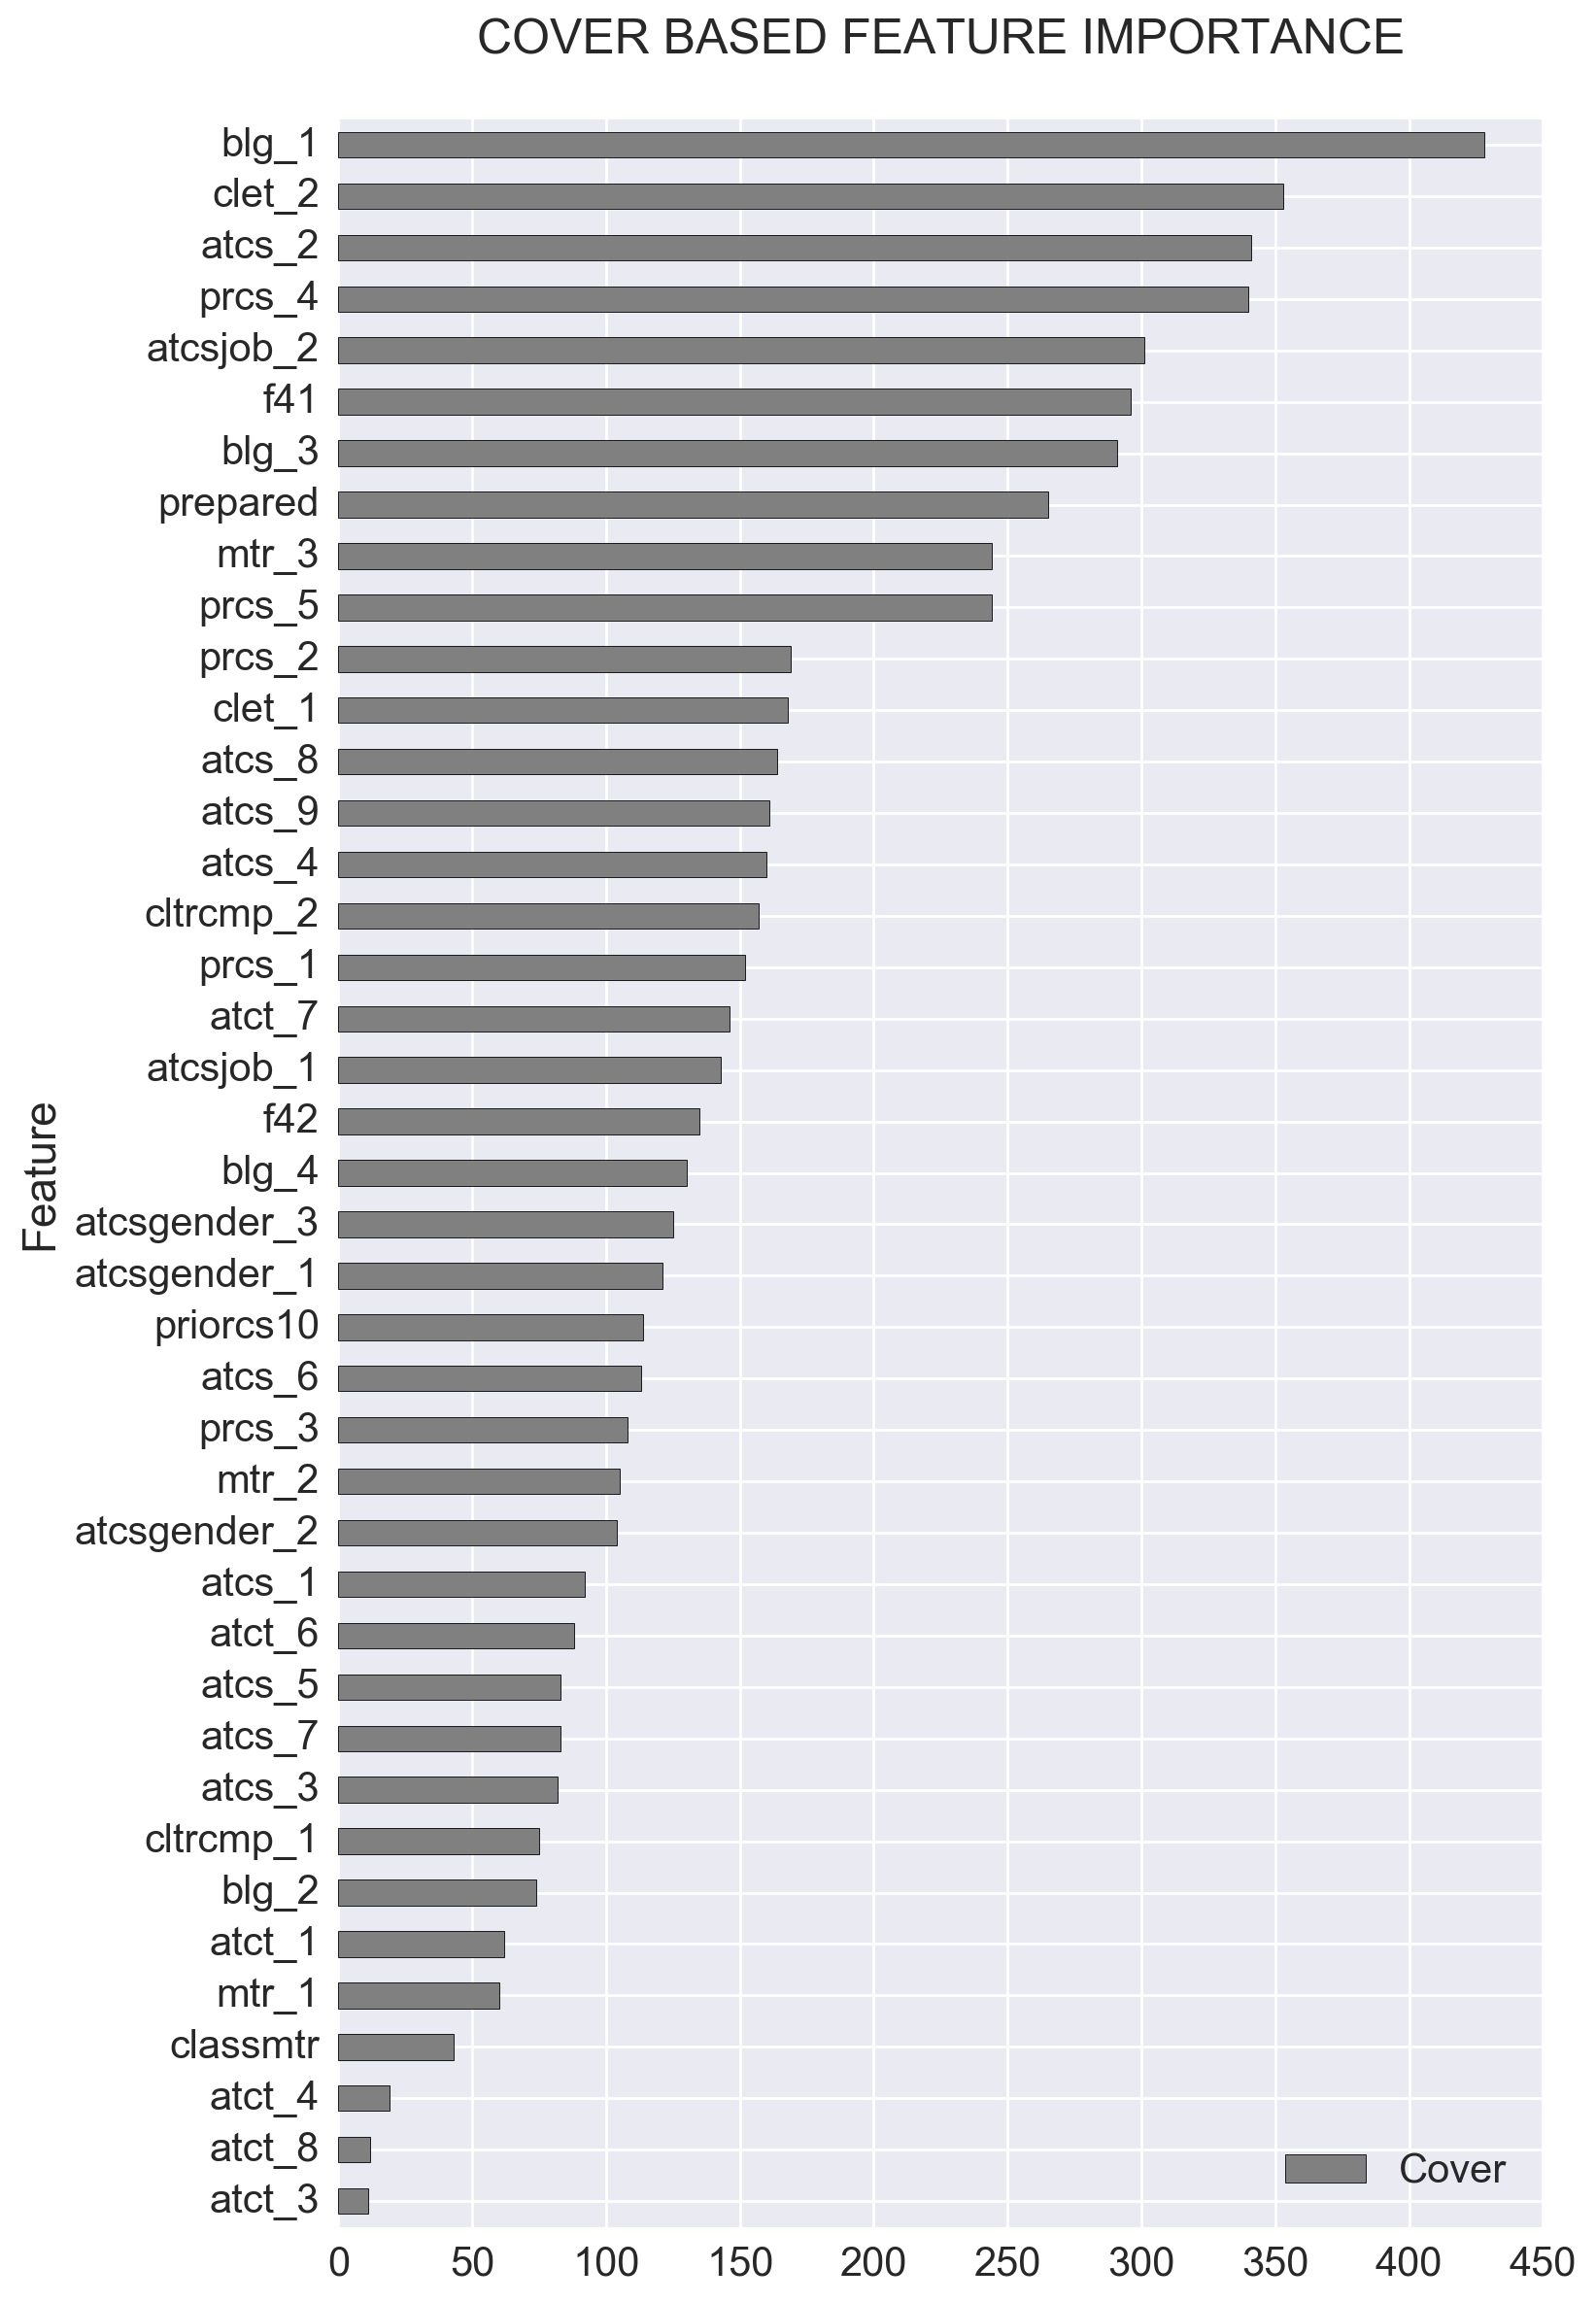
\includegraphics[width=0.6\textwidth]{figures/featureImportance_cover}
    \label{f_imp}}
    \subfloat[Feature Importance Based on Information Gain]{%
    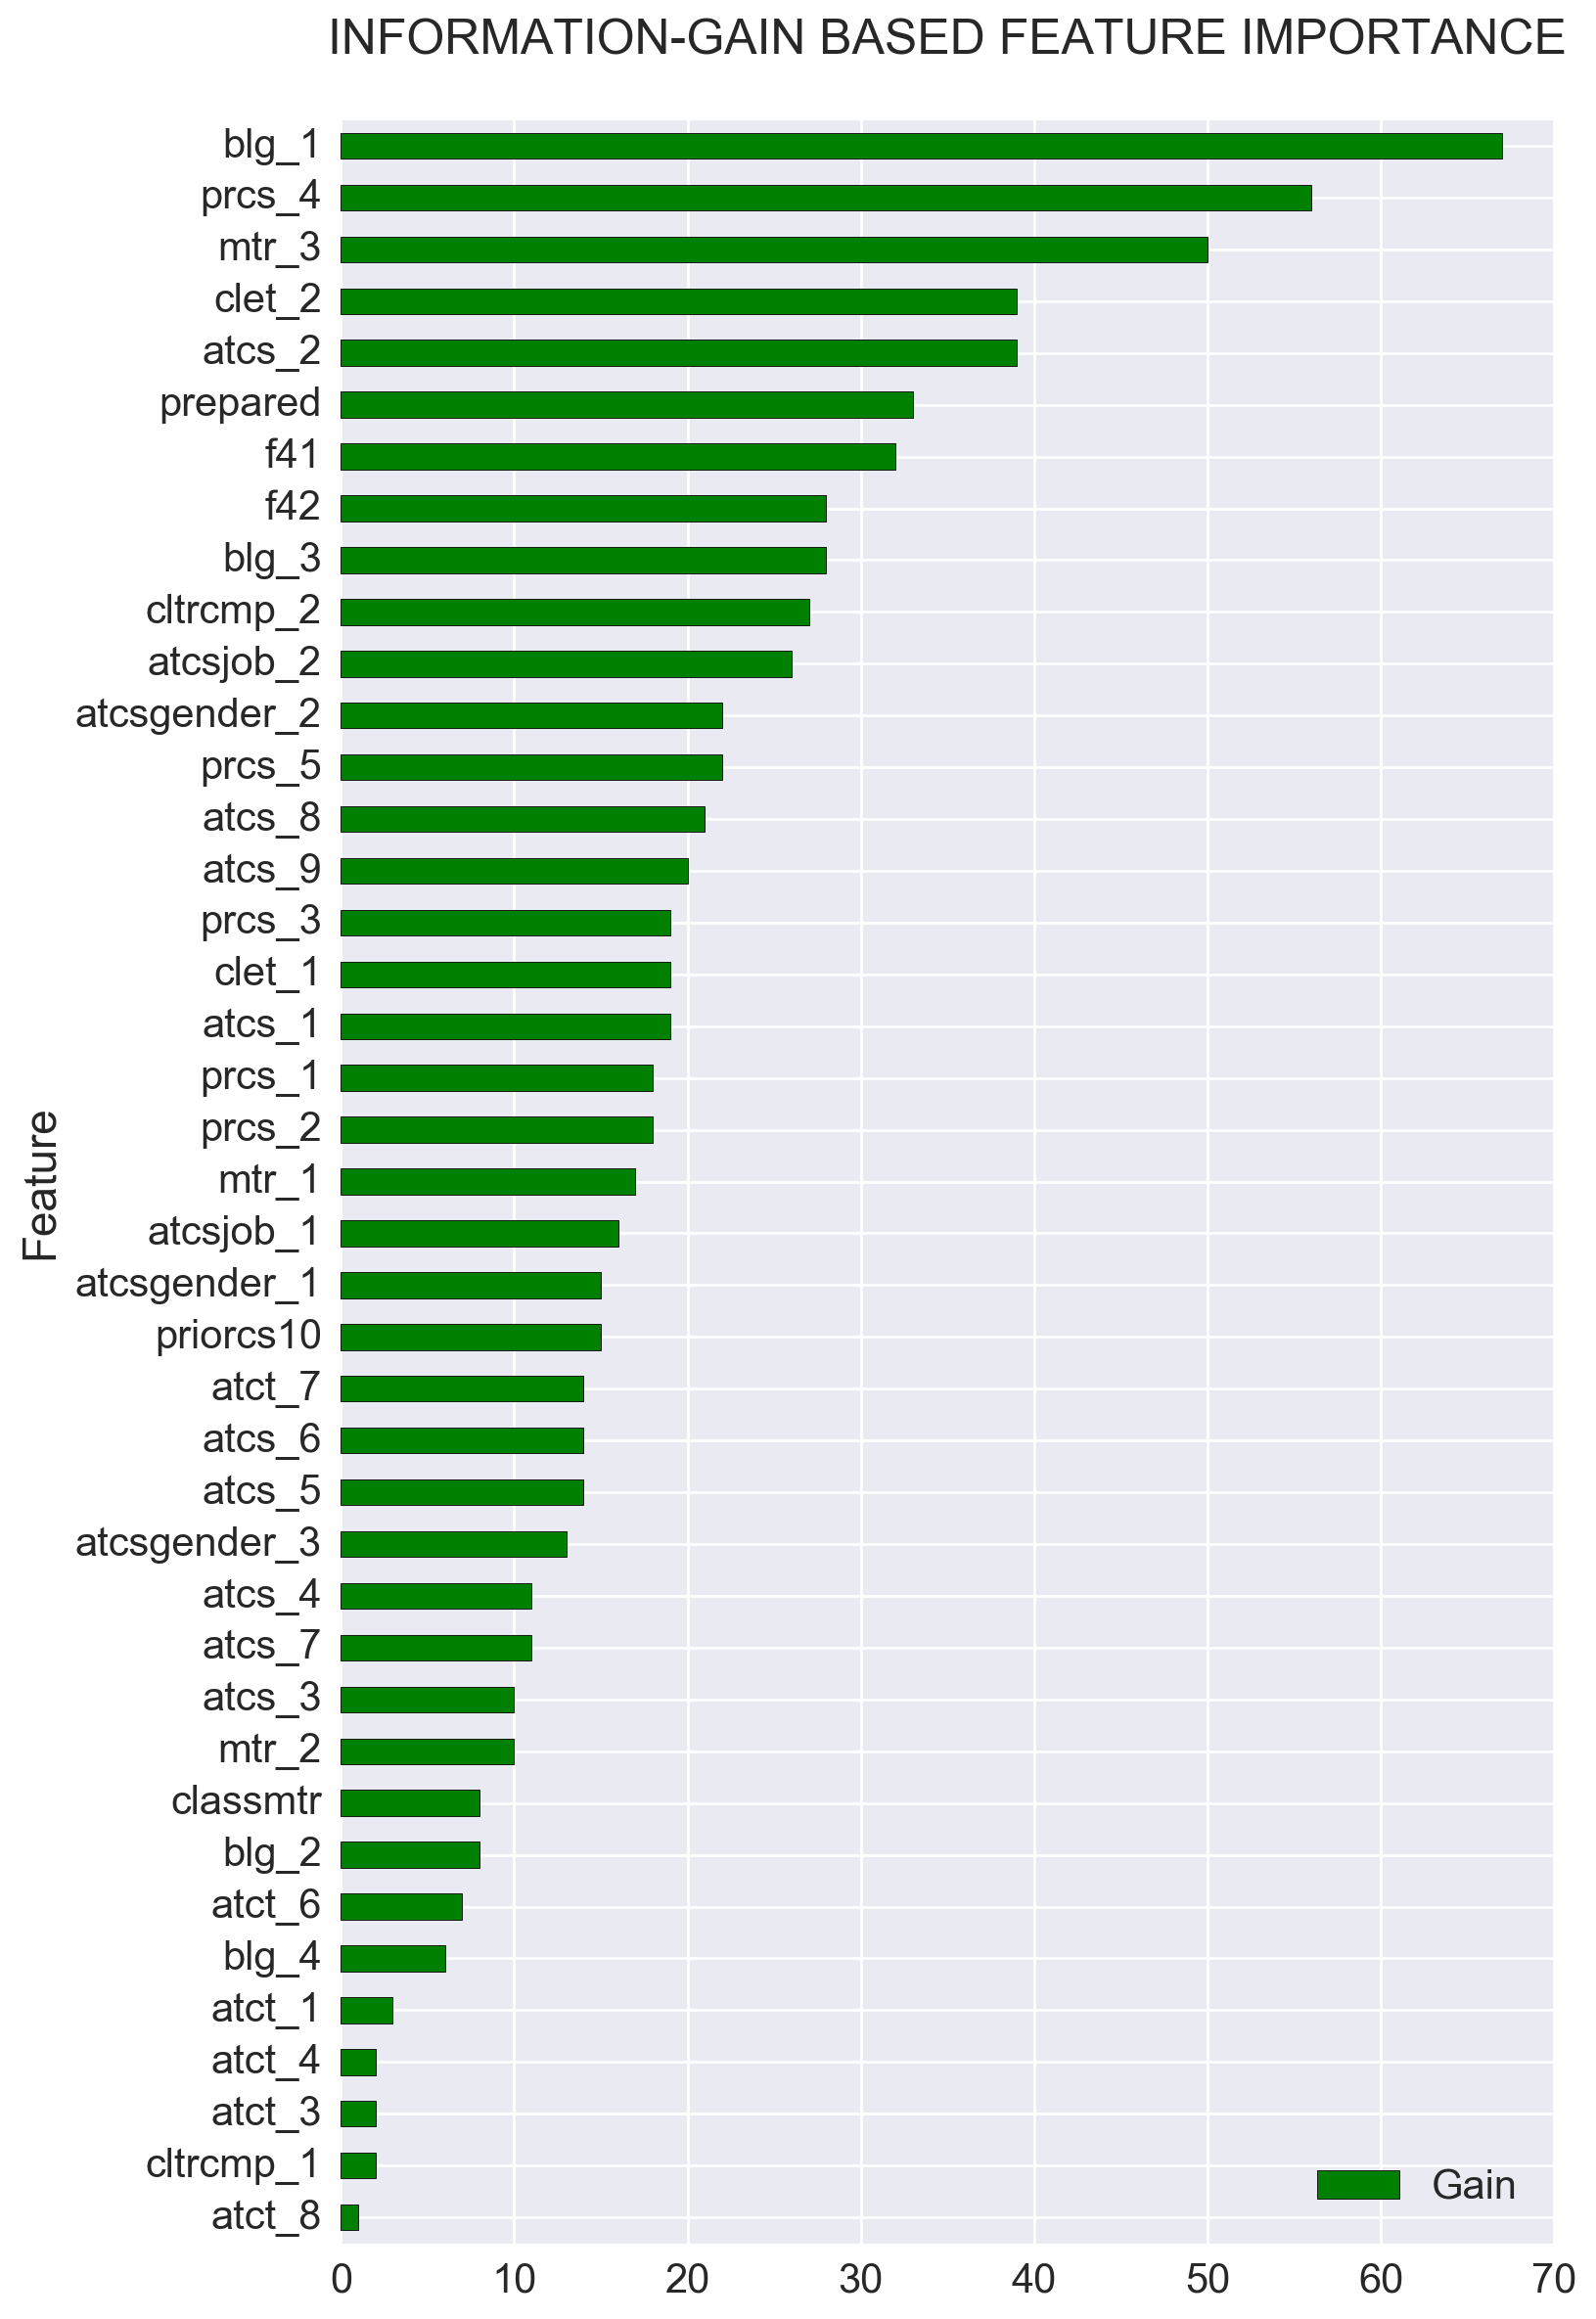
\includegraphics[width=0.6\textwidth]{figures/featureImportance_informationGain}
    \label{f_imp_tuned}}

    \caption{\textbf{XgBoost Feature Importance}}
\end{figure}


%----------------------------------------------------------------------------------------
%  CHAPTER 
%----------------------------------------------------------------------------------------

\chapter*{Conclusion}



\section*{Reflection}

